\documentclass[12pt,a4paper]{article}
\usepackage[UTF8]{ctex}
\usepackage{geometry}
\usepackage{graphicx}
\usepackage{booktabs}
\usepackage{multirow}
\usepackage{array}
\usepackage{float}
\usepackage{listings}
\usepackage{xcolor}
\usepackage{fancyhdr}
\usepackage{titlesec}
\usepackage{setspace}
\usepackage{amsmath}
\usepackage{amssymb}
\usepackage{lastpage}
\usepackage{tabularx}
\usepackage{threeparttable}
\usepackage{tikz}
\usetikzlibrary{graphs, positioning, arrows.meta}
\geometry{margin=2.5cm}


\usepackage{subcaption}
% \usepackage[hidelinks]{hyperref}   % 隐藏链接颜色框，但保留跳转
\usepackage{hyperref}
\hypersetup{
    colorlinks=true,
    linkcolor=ccr,
    anchorcolor=ccr,
    citecolor=ccr}
\definecolor{ccr}{RGB}{10,110,150}

% 页面设置
\geometry{a4paper,left=2.5cm,right=2.5cm,top=2.5cm,bottom=2.5cm}
\setlength{\parskip}{0.5em}
\setlength{\headheight}{14.49998pt}
\addtolength{\topmargin}{-2.49998pt}
\onehalfspacing

% 页眉页脚设置
\pagestyle{fancy}
\fancyhf{}
\fancyhead[L]{中山大学计算机学院}
\fancyhead[C]{FoodFlow：外卖三方推荐与动态履约仿真}
\fancyhead[R]{}
\fancyfoot[C]{\thepage\ /\ \pageref{LastPage}}
\renewcommand{\headrulewidth}{0.4pt}
\renewcommand{\footrulewidth}{0.4pt}

% 标题格式设置
\titleformat{\section}{\Large\bfseries}{\thesection}{1em}{}
\titleformat{\subsection}{\large\bfseries}{\thesubsection}{1em}{}
\titleformat{\subsubsection}{\normalsize\bfseries}{\thesubsubsection}{1em}{}

% 代码样式设置
\lstset{
    backgroundcolor=\color{gray!10},
    basicstyle=\ttfamily\footnotesize,
    breaklines=true,
    frame=single,
    numbers=left,
    numberstyle=\tiny\color{gray},
    keywordstyle=\color{blue},
    commentstyle=\color{green!60!black},
    stringstyle=\color{red},
    showstringspaces=false,
    tabsize=4
}

\begin{document}

% 封面页
\begin{titlepage}
	\centering
	\vspace*{1cm}
	
\includegraphics[width=0.6\textwidth]{pc1.png}
	\paragraph{}
	{\Huge\bfseries\
		本科生实验报告\par}
	\vspace{4cm}
	\begin{center}
		\hspace*{4.8em}
		{\Large
			\begin{tabular}{rl}
				实验课程： & 大数据原理与技术 \\
				实验名称： & 外卖三方推荐与动态履约仿真系统 \\
				专业名称： & 计算机科学与技术 \\
				实验地点： & 东校园实验中心大楼 B201 \\
				报告时间： & 2026/7/6\\
			\end{tabular}\par}
	\end{center}
	\vspace{2cm}
	\newcolumntype{C}{>{\centering\arraybackslash}X}
	
	\begin{tabularx}{\textwidth}{|c|C|C|C|C|}
		\hline
		组员 & 成员1 & 成员2 & 成员3 & 成员4 \\ \hline
		学号 & 23342035 & 23336011 & 23336003 & 23320143 \\ \hline
		姓名 & 黄镇邦 & 谭栋泽 & 陈政宇 & 唐雅妍 \\ \hline
	\end{tabularx}
	\vfill
\end{titlepage}

    % 目录
    \tableofcontents
    \newpage

    \section{实验目的}

    本实验旨在构建一个面向外卖平台的推荐与动态履约仿真系统 FoodFlow。外卖推荐不能仅追求 Recall 或 NDCG——推荐列表会改变订单的空间分布，进而影响商家曝光、骑手负载、预计送达时间（ETA）和超时风险。因此 FoodFlow 在用户偏好之外，引入商家公平、ETA、供给约束和骑手负载，将推荐系统扩展为"用户—商家—骑手"三方闭环。

    实验目标包括：
    \begin{enumerate}
        \item 基于真实外卖订单数据（TRD 数据集），实现多种推荐模型，包括协同过滤、序列推荐、学习排序（LTR）以及三方重排方法；
        \item 构建动态履约仿真器，将推荐结果转化为模拟订单，接入骑手匹配与高峰期履约仿真；
        \item 通过离线评估指标（Recall、NDCG、Coverage、Exposure Gini 等）和仿真指标（平均 ETA、超时率、平台效用等），综合评估不同策略在三方指标上的权衡。
    \end{enumerate}

    \paragraph{} % 空行
    \paragraph{} % 空行

    \section{实验过程和核心代码}

    \subsection{数据来源与预处理}

    主数据集为 Takeout Recommendation Dataset (TRD)，DOI：\texttt{10.5281/zenodo.8025855}。数据来自美团外卖北京 11 个商圈，时间范围为 2021-03-01 至 2021-03-28，包含用户、餐厅、菜品、训练订单、测试订单和测试标签。项目默认下载 TRD 的 txt 文件，训练集使用完整 \texttt{orders\_train.txt}。

    数据审计结果如表 \ref{tab:data_audit} 所示。

    \begin{table}[h]
        \centering
        \caption{TRD 数据集审计结果}
        \label{tab:data_audit}
        \begin{tabular}{lr}
            \toprule
            \textbf{审计项目} & \textbf{数值} \\
            \midrule
            必需 TRD 文件齐全 & 是 \\
            训练集处理模式 & full \\
            原始训练订单数 & 1,068,495 \\
            处理后训练订单数 & 1,068,495 \\
            训练订单使用比例 & 1.0000 \\
            用户数 & 200,000 \\
            商家数 & 29,072 \\
            测试订单数 & 230,550 \\
            离线评估用户数 & 300（前 300 名测试用户） \\
            \bottomrule
        \end{tabular}
    \end{table}

    TRD 不包含真实骑手数据，因此骑手位置、在线状态、负载和收入基于固定 seed 合成代理数据。可使用 LaDe delivery CSV 校准骑手速度、服务时长和负载分布，但 LaDe 并非外卖平台数据。

    \subsection{推荐模型设计}

    系统实现了 8 个代表性推荐策略，涵盖从简单基线到知识图谱增强的不同层次：

    \textbf{Popular（全局热门基线）：}按商家历史订单量排序，作为无个性化的对照组。

    \textbf{BPR-MF（贝叶斯个性化排序矩阵分解）：}基于用户-商家隐式反馈，使用 24 维潜在因子、4 个 epoch 的 SGD 训练，是传统协同过滤的经典实现。

    \textbf{UserOnly（基于用户画像的可解释排序）：}综合品类偏好（权重 0.20）、复购（0.52）、价格匹配（0.10）、时段偏好（0.06）、商家质量（0.07）和新颖度（0.05），构造完全可解释的推荐分数。

    \textbf{Seq-Tuned（序列混合推荐）：}基于用户最近下单序列，提取快慢时间衰减、复购、商家转移、品类偏好、热度和质量等七类序列特征，通过人工调优的权重进行加权融合。权重配置为近因性（0.143+0.094）、复购（0.412）、转移（0.247）、品类（0.091）、热度（0.009）、质量（0.004）。

    \textbf{LightGBM-LTR（LambdaRank 学习排序）：}复用 Seq-Tuned 的七类序列特征，使用 LightGBM LambdaRank 学习非线性排序函数，替代手工设定的权重。当 LightGBM 不可用时，自动回退为 Logistic-LTR。

    推荐模型的候选集生成遵循以下流程：首先对每个用户提取历史下单序列和商家频次，计算七类序列特征值；然后基于特征分数对候选商家进行初筛，保留前 80 名进入重排阶段。核心特征计算公式如下：

    对于复购特征（repeat），定义用户 $u$ 对商家 $m$ 的复购分为：
    \begin{equation}
        \text{repeat}(u, m) = \frac{\ln(1 + \text{count}(u, m))}{\ln 5}
    \end{equation}
    其中 $\text{count}(u, m)$ 为用户 $u$ 在训练集中下单商家 $m$ 的总次数。

    对于商家转移特征（transition），考虑用户序列中从商家 $m_i$ 到 $m_j$ 的转移概率：
    \begin{equation}
        \text{transition}(u, m) = \frac{\sum_{t=1}^{|\text{seq}|-1} \mathbb{I}[\text{seq}_t = m_{\text{prev}}] \cdot \text{cooccur}(m_{\text{prev}}, m)}{\max(1, |\text{seq}|-1)}
    \end{equation}

    \textbf{Seq-xQuAD-Tripartite（序列推荐 + 三方重排）：}在 Seq-Tuned 候选集基础上，引入三方重排架构。候选集经过 min-max 归一化后，加权合成四个分量：用户偏好分（user\_score，权重 0.93）、商家公平分（fairness，权重 0.025）、ETA 分（eta\_score，权重 0.03）和供给分（supply\_score，权重 0.015）。之后通过 xQuAD 算法进行逐步选择，平衡相关性（权重 0.84）、品类覆盖多样性（0.12）和长尾曝光（0.04）。

    \textbf{Session-SPU-Tripartite（会话与菜品增强三方）：}在三方重排基础上，额外注入训练期会话点击候选和基于 SPU 菜品品类的商家亲和度。通过菜品品类重叠扩展候选集，session 权重为 0.055，spu 权重为 0.015。

    \textbf{KG-Tripartite（知识图谱增强三方推荐）：}在三方重排架构之上，引入轻量知识图谱兴趣信号。该模型不训练完整图神经网络，而是将 TRD 结构化字段（商家类目、商圈区域、价格段、评分等级、口味、食材、品牌等）组织为知识图谱三元组，通过时间衰减将用户历史订单转化为图谱上的带权兴趣边（历史偏好边 \texttt{pref\_hist} 和点击临时兴趣边 \texttt{pref\_click}），在候选排序中叠加图谱路径匹配特征。KG-Tripartite 的完整动态 KG 注意力模型（torch 实现与 GPU 实验结果）见 \texttt{kg-demo/} 子项目，包含关系感知图注意力聚合、LightGCN 基础实现和 Final Hybrid 融合方案；主项目中的 KG-Tripartite 是其免训练的轻量近似版本，通过时间衰减与关系加权匹配将图谱信号接入三方重排，并可从历史下单、品类、区域和价格段构造路径证据解释推荐原因。

    \subsection{三方重排架构}

    三方重排是 FoodFlow 的核心创新点，其架构如图 \ref{fig:framework} 所示。

    \begin{figure}[htbp]
        \centering
        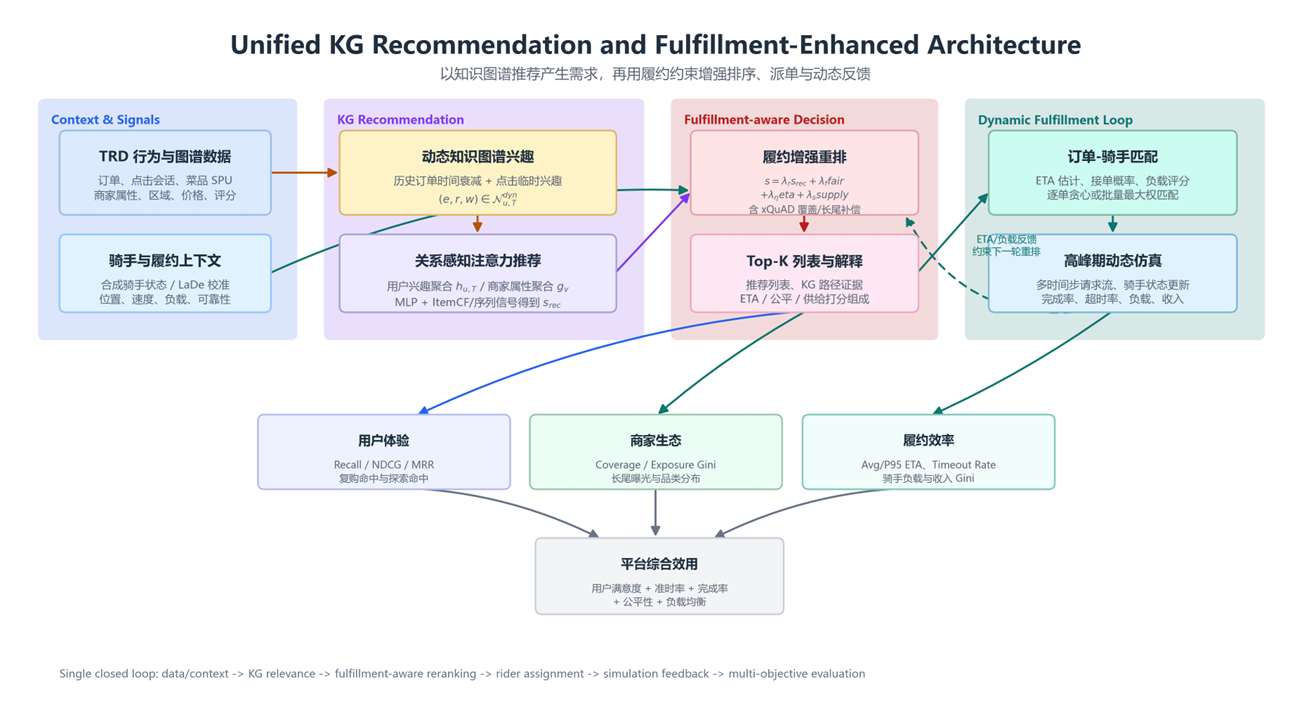
\includegraphics[width=0.9\textwidth]{framework.png}
        \caption{FoodFlow 系统架构图}
        \label{fig:framework}
    \end{figure}
    % \begin{figure}[htbp]
    %     \centering
    %     \begin{tikzpicture}[node distance=1.8cm, auto,
    %         block/.style={rectangle, draw, fill=blue!10, text width=6cm, text centered, minimum height=0.8cm, rounded corners},
    %         data/.style={rectangle, draw, fill=gray!10, text width=4cm, text centered, minimum height=0.7cm},
    %         arrow/.style={-{Stealth[scale=1.2]}, thick}]

    %         % 数据层
    %         \node[data] (trd) {TRD 真实订单数据};
    %         \node[block, above=0.8cm of trd] (preprocess) {预处理与特征工程};
    %         \node[data, above=0.8cm of preprocess, text width=7cm] (features) {用户画像 / 商家特征 / 序列特征 / 上下文};

    %         % 推荐层
    %         \node[block, above=1.2cm of features, fill=yellow!15, text width=8cm] (recall) {\textbf{召回与基础排序层} \\ Popular / BPR-MF / UserOnly / Seq-Tuned / LightGBM-LTR};

    %         % 重排层
    %         \node[block, above=1.2cm of recall, fill=green!10, text width=10cm] (rerank) {\textbf{三方重排层 (xQuAD)} \\[2pt]
    %             \footnotesize 候选集 Min-Max 归一化 $\rightarrow$ 分数融合 $\rightarrow$ xQuAD 逐步选择 \\[2pt]
    %             \footnotesize 用户分(0.93) + 公平分(0.025) + ETA分(0.03) + 供给分(0.015)};

    %         % 仿真层
    %         \node[block, above=1.2cm of rerank, fill=red!10, text width=8cm] (sim) {\textbf{动态履约仿真层} \\ 骑手匹配（贪心/二分图批量）+ 状态更新};

    %         % 输出
    %         \node[data, above=0.8cm of sim, text width=8cm] (output) {最终推荐列表 + 履约指标};

    %         % 连线
    %         \draw[arrow] (trd) -- (preprocess);
    %         \draw[arrow] (preprocess) -- (features);
    %         \draw[arrow] (features) -- (recall);
    %         \draw[arrow] (recall) -- (rerank);
    %         \draw[arrow] (rerank) -- (sim);
    %         \draw[arrow] (sim) -- (output);
    %     \end{tikzpicture}
    %     \caption{FoodFlow 系统架构图}
    %     \label{fig:framework}
    % \end{figure}

    三方分数融合的具体计算方式如下：对于给定的候选商家集合 $\mathcal{C}$，首先对各分量的原始值进行 min-max 归一化，得到归一化分数 $\tilde{s}_u(m)$（用户分）、$\tilde{s}_f(m)$（公平分）、$\tilde{s}_e(m)$（ETA分）和 $\tilde{s}_s(m)$（供给分）。三方总分由加权和给出：
    \begin{equation}
        s_{\text{tri}}(m) = w_u \cdot \tilde{s}_u(m) + w_f \cdot \tilde{s}_f(m) + w_e \cdot \tilde{s}_e(m) + w_s \cdot \tilde{s}_s(m)
    \end{equation}
    其中权重满足 $w_u + w_f + w_e + w_s = 1$。

    商家公平分的定义为 $s_f(m) = 0.75 \cdot (1 - \text{norm\_pop}(m)) + 0.25 \cdot \text{quality}(m)$，即对高曝光商家进行惩罚、对高质量低曝光商家进行补偿。ETA 分定义为 $s_e(m) = 1.0 - \min(\text{eta}(m) / 70.0,\ 1.0)$。供给分定义为 $s_s(m) = 0.6 \cdot (\text{delivery\_score}(m) / 5.0) + 0.4 / (1 + \ln(1 + \text{order\_count}(m)))$，综合考虑商家配送能力和长尾供给。

    xQuAD 逐步选择的每一步中，对每个未被选中的候选商家 $m$，计算其综合价值：
    \begin{equation}
        v(m) = \lambda_r \cdot \text{rel}(m) + \lambda_d \cdot \text{div}(m) + \lambda_t \cdot \text{tail}(m)
    \end{equation}
    其中 $\text{rel}(m)$ 为归一化后的三方总分，$\text{div}(m) \in \{0, 1\}$ 表示该商家品类是否尚未被已选列表覆盖，$\text{tail}(m) = 1/(1 + \ln(1 + \text{order\_count}(m)))$ 为长尾奖励。

    \subsection{动态履约仿真}

    仿真参数配置为：8 个时间步 $\times$ 每步 16 个请求 = 128 个请求/策略，Top-K = 10，模拟午餐高峰时段（每步间隔 5 分钟）。仿真流程如下：

    \begin{enumerate}
        \item 为当前策略拟合推荐器；
        \item 使用固定种子生成 120 个合成骑手；
        \item 对于每个时间步：
        \begin{itemize}
            \item 更新骑手可用性（减少负载，标记空闲骑手）；
            \item 从评估用户中抽样请求用户；
            \item 运行推荐器，获取每个用户的 Top-K 推荐；
            \item 基于 MNL/Softmax 选择模型模拟用户决策；
            \item 根据派单策略分配订单给骑手；
            \item 更新骑手状态（位置、负载、收入）。
        \end{itemize}
        \item 收集每个策略的最终指标。
    \end{enumerate}

    \subsubsection{MNL 用户选择模型}

    用户根据效用函数从推荐列表中选择商家，公式如下：
    \begin{equation}
        U(m) = -0.45 + \alpha_s \cdot \tilde{s}(m) + \alpha_r \cdot r(m) + \alpha_t \cdot \mathbb{I}[m \in \mathcal{T}_u]
    \end{equation}
    其中 $\tilde{s}(m)$ 为归一化推荐分数，$r(m) = 1/\log_2(\text{rank}(m) + 1)$ 为排名先验，$\mathbb{I}[m \in \mathcal{T}_u]$ 为真实命中奖励（bonus = 1.75）。不作选择的效用设为 2.0。选择概率由 Softmax 给出。

    \subsubsection{骑手配送策略}

    系统实现了四种骑手派单策略，如表 \ref{tab:rider_policies} 所示。

    \begin{table}[h]
        \centering
        \caption{骑手派单策略}
        \label{tab:rider_policies}
        \begin{tabular}{lll}
            \toprule
            \textbf{策略名称} & \textbf{分配方式} & \textbf{核心逻辑} \\
            \midrule
            nearest & 贪心 & 选择接驾距离最小的骑手 \\
            min\_eta & 贪心 & 选择 ETA 最小的骑手 \\
            load\_aware greedy & 贪心 & 负载感知评分，逐单分配 \\
            load\_aware batch & 批量最优 & 负载感知 + 容量槽位二分图匹配 \\
            \bottomrule
        \end{tabular}
    \end{table}

    \subsection{二分图匹配派单算法}

    对于批量派单模式，在每个时间步将所有待分配订单与骑手容量槽位构成二分图，使用匈牙利算法求最大权匹配。算法流程如下：

    \textbf{步骤一：构建容量槽位。}对于每个骑手 $r_i$，其当前负载为 $l_i$，最大负载为 $L_{\max} = 3$，则创建 $c_i = \max(0, L_{\max} - l_i)$ 个容量槽位。每个槽位对应一个虚拟节点，允许同一个骑手接收多笔订单。

    \textbf{步骤二：构建评分矩阵。}设订单数为 $N_o$，槽位总数为 $N_s$，构造评分矩阵 $S \in \mathbb{R}^{N_o \times N_s}$，其中：
    \begin{equation}
        S_{ij} = \text{rider\_score}(\text{eta}_{ij}, r_j, \text{accept}_{ij}) - 0.20 \cdot \text{timeout\_risk}_{ij}
    \end{equation}
    骑手得分的计算为：
    \begin{equation}
        \text{rider\_score} = 0.50 \cdot s_{\text{eta}} + 0.20 \cdot s_{\text{reliability}} + 0.15 \cdot s_{\text{load}} + 0.15 \cdot s_{\text{accept}}
    \end{equation}
    其中 $s_{\text{eta}} = 1.0 - \min(\text{eta} / 70.0, 1.0)$，$s_{\text{reliability}}$ 基于骑手历史准时率，$s_{\text{load}} = 1.0 - \min(l / L_{\max}, 1.0)$，$s_{\text{accept}}$ 为骑手接单概率估计。超时风险惩罚项定义为 $\text{timeout\_risk} = \min(\max((\text{eta} - 45.0) / 60.0, 0.0), 1.0)$。

    \textbf{步骤三：匈牙利算法求解。}调用 \texttt{scipy.optimize.linear\_sum\_assignment} 对负评分矩阵 $-S$ 求最小代价分配，等价于原始问题的最大权匹配。过滤掉匹配得分极低（$\leq -10^5$）的分配结果。

    \textbf{步骤四：执行分配并更新骑手状态。}将匹配成功的订单分配给对应骑手，更新骑手位置、负载和收入。每位骑手的收入由基础配送费与距离补偿构成：$\text{income} = 5.0 + \text{eta} \times 0.08$。

    \subsection{ETA 估计模型}

    预计配送时间（ETA）由以下分量构成：
    \begin{equation}
        \text{ETA} = t_{\text{wait}} + t_{\text{prep}} + t_{\text{peak}} + \frac{d_{\text{rider}\to\text{store}}}{\text{pickup\_speed}} \times 60 + \frac{d_{\text{store}\to\text{user}}}{\text{delivery\_speed}} \times 60 + t_{\text{load}}
    \end{equation}
    其中 $t_{\text{prep}} = \text{service\_minutes} + (1 - \text{food\_score}/5) \times 5$（商家备餐时间），$t_{\text{peak}}$ 在高峰期加 6 分钟、非高峰期加 2 分钟，$t_{\text{load}} = \text{current\_load} \times 5$（骑手当前负载惩罚），配送速度 = 取餐速度 $\times 1.08$。

    \subsection{平台效用函数}

    综合平台效用函数被定义为各维度指标的加权和，用于从全局视角评估策略的系统级表现：
    \begin{equation}
        \begin{aligned}
            U_{\text{platform}} = 0.25 \cdot s_{\text{user}} &+ 0.25 \cdot r_{\text{ontime}} + 0.20 \cdot r_{\text{complete}} \\
            &+ 0.15 \cdot (1 - g_{\text{merchant}}) + 0.10 \cdot (1 - \text{cv}_{\text{rider}}) - 0.05 \cdot r_{\text{timeout}}
        \end{aligned}
    \end{equation}
    其中 $s_{\text{user}}$ 为用户满意度，$r_{\text{ontime}}$ 为准时率，$r_{\text{complete}}$ 为订单完成率，$g_{\text{merchant}}$ 为商家曝光 Gini 系数，$\text{cv}_{\text{rider}}$ 为骑手负载变异系数，$r_{\text{timeout}}$ 为超时率。该效用函数兼顾了用户体验、配送效率和生态公平三个维度。

    \subsection{知识图谱增强与可解释推荐}

    FoodFlow 的轻量 KG 模块（\texttt{foodflow/kg.py}）不训练 LightGCN/KGAT 等完整图神经网络，而是将现有结构化字段转化为知识图谱三元组和可解释推荐路径。与此同时，\texttt{kg-demo/} 子项目提供了完整的动态知识图谱注意力模型（torch 实现与 GPU 实验），包含关系感知图注意力聚合、时间衰减动态边权、临时兴趣节点和 Final Hybrid 融合方案，下文一并介绍。

    \subsubsection{知识图谱实体与关系设计}

    知识图谱实体包括：用户实体、商家实体、餐饮类目实体（一/二/三级）、口味实体（由菜品 taste 字段抽取）、食材实体、价格区间实体（由订单价格聚合）、评分等级实体（离散为 low/medium/high/excellent）、区域实体（aor\_id）、品牌实体和标准菜品实体。静态三元组以商家为头实体、属性为尾实体，关系包括 \texttt{has\_cat1/2/3}、\texttt{has\_brand}、\texttt{located\_in\_aor}、\texttt{has\_price}、\texttt{has\_poi\_score}、\texttt{has\_delivery\_score}、\texttt{has\_food\_score}、\texttt{has\_ingredient}、\texttt{has\_taste}、\texttt{has\_standard\_food} 等。主项目轻量 KG 共导出约 24 万条静态三元组。

    \subsubsection{动态图谱构造：时间衰减与临时兴趣}

    设用户 $u$ 在时间 $t$ 与商家 $i$ 发生过订单交互，当前推荐请求时间为 $T$。历史订单边权采用指数衰减 $w_{u,i,t}=\exp(-\lambda (T-t))$，其中 $\lambda=0.12$ 为衰减系数（以天为单位）。用户对兴趣实体 $e$ 的历史偏好为 $p^{hist}_{u,e}=\sum_{(i,t)\in \mathcal{H}_{u,T}} w_{u,i,t} A_{i,e}$，其中 $A_{i,e}=1$ 表示商家 $i$ 与实体 $e$ 通过静态图谱相连。

    下单前点击序列反映当前一餐的短期偏好。设点击序列为 $\mathcal{C}_{u,T}=(c_1,c_2,\ldots,c_m)$，越靠近下单的点击权重越高：$w^{click}_{u,c_j,T}=\eta \rho^{m-j}$（$\eta=1.6,\ \rho=0.88$）。点击序列生成的临时偏好为 $p^{click}_{u,e}=\sum_{c_j\in \mathcal{C}_{u,T}} w^{click}_{u,c_j,T} A_{c_j,e}$。最终动态图谱邻居集合合并两类偏好边：$\mathcal{N}^{dyn}_{u,T}=\{(e,\texttt{pref\_hist},p^{hist}_{u,e})\}\cup\{(e,\texttt{pref\_click},p^{click}_{u,e})\}$。

    \subsubsection{关系感知图注意力模型（kg-demo 完整版）}

    kg-demo 子项目实现了完整的关系感知图注意力模型。记用户 embedding 为 $\mathbf{q}_u$，兴趣实体 embedding 为 $\mathbf{e}_e$，关系 embedding 为 $\mathbf{r}$，动态偏好权重为 $p_{u,e}$。注意力分数为 $s_{u,e,r}=\mathbf{a}^{\top}\tanh(W_q\mathbf{q}_u+W_e\mathbf{e}_e+W_r\mathbf{r})+\beta\log(1+p_{u,e})$，其中 $\log(1+p_{u,e})$ 将时间衰减或点击临时偏好作为 softmax 偏置。用户当前兴趣表示为 $\mathbf{h}_{u,T}=\mathrm{LayerNorm}(\mathbf{q}_u+\sum_{(e,r)}\alpha_{u,e,r}(\mathbf{e}_e+\mathbf{r}))$。排序层采用 MLP，将动态图谱用户表示、候选商家图谱表示、二者逐元素乘积以及基础特征拼接：$\mathrm{score}(u,v,T)=\mathrm{MLP}([\mathbf{h}_{u,T},\mathbf{g}_v,\mathbf{h}_{u,T}\odot \mathbf{g}_v,\mathbf{x}_{u,v,T}])$。

    在 TRD 10 万订单子集（200 候选 sampled ranking）上的实验表明，该完整模型的 Final Hybrid（与 ItemCF 分数查询内标准化后线性融合）取得最佳结果：Recall@5=0.157、Recall@10=0.210、Recall@20=0.294、NDCG@10=0.147、AUC=0.702，说明协同过滤邻域信号与动态图谱短期兴趣信号具有互补性。

    \subsubsection{轻量 KG 路径解释}

    主项目 \texttt{foodflow/kg.py} 将结构化字段转成可解释路径，例如：用户 $\rightarrow$ 历史下单商家 $\rightarrow$ 商家；用户 $\rightarrow$ 偏好品类 $\leftarrow$ 候选商家；用户 $\rightarrow$ 下单区域 $\leftarrow$ 候选商家；用户 $\rightarrow$ 价格段 $\leftarrow$ 候选商家。这些路径来自训练订单、用户品类偏好、商家类目、商家区域和价格段等真实字段。KG-Tripartite 在推荐时会将路径证据、ETA 和曝光补偿一起输出，保证解释引用真实参与推荐/重排的数据。

    \subsection{路径感知顺路派单}

    除传统的最近骑手、最小 ETA 和负载感知逐单/批量匹配外，FoodFlow 新增了路径感知顺路派单策略。骑手不再只按直线距离或单点 ETA 评估，而是维护取/送航点序列（route），新单按 cheapest-insertion 算法枚举所有（取餐点，送达点）插入位置，计算边际绕行分钟数：

    \begin{itemize}
        \item \textbf{RouteMinETA：}在路径机制下最小化该单 ETA，作为 route 家族的公平基线。
        \item \textbf{RouteBatch（RouteInsertion）：}目标为边际绕行 + ETA（等权），批量版按匈牙利轮次匹配，每轮每骑手至多一单，应用插入后重算下一轮成本。
    \end{itemize}

    骑手随时间沿路径行进（每步推进 5 分钟，经过 dropoff 即完成一单），替代"派单即瞬移"的简化假设。新增指标包括平均边际绕行（avg\_detour\_minutes）和顺路接单率（enroute\_pickup\_share）。

    \subsection{真实城市地理编码}

    TRD 不含坐标，旧实现用高斯随机数合成经纬度。现在通过 \texttt{make geocode} 将用户/商家嵌入 LaDe（Cainiao 末端配送数据集）真实城市的配送 GPS 分布：先粗聚类提取最大密度簇质心 10km 内的城市核心区；每个 aor\_id 商圈映射到真实高密度簇，商家坐标从簇内真实点采样（约 60m 抖动）；每个 aoi\_id 居住区取真实锚点，用户在 120m 内散布。元数据写入 \texttt{data/processed/geo\_note.json}。诚实口径：这不是 TRD 的真实位置，而是"TRD 订单嵌入 LaDe 真实城市空间分布"；但从此距离、ETA 与地图展示具备真实街区尺度。所有行程按直线距离 $\times 1.3$ 道路弯曲系数换算，骑手默认速度校到 25 km/h（电动车市区口径）；备餐与骑手赶往商家并行计时，使 ETA 尺度落在合理区间。

    \section{实验结果}

    \subsection{离线推荐结果}

    离线评估使用前 300 名测试用户，评估指标包括推荐侧（Recall@K、NDCG@K、MRR@K、HitRate@K）、商家侧（Coverage@20、Exposure Gini、LongTailExposure@20）和校准侧（CategoryJSD@20）。
    各模型在 $K=20$ 下的主要指标如表 \ref{tab:offline_accuracy} 和 \ref{tab:offline_diversity} 所示。

    \begin{table}[htbp]
        \centering
        \caption{离线推荐准确性指标（$K=20$）}
        \label{tab:offline_accuracy}
        \begin{tabular}{lcc}
            \toprule
            \textbf{模型} & \textbf{Recall@20} & \textbf{NDCG@20} \\
            \midrule
            Popular & 0.0470 & 0.0210 \\
            BPR-MF & 0.1620 & 0.1068 \\
            UserOnly & 0.4287 & 0.3423 \\
            KG-Tripartite & 0.4263 & 0.3480 \\
            Logistic-LTR & 0.4013 & 0.3412 \\
            \textbf{Seq-Tuned} & \textbf{0.4675} & \textbf{0.3652} \\
            Seq-xQuAD-Tripartite & 0.4113 & 0.3426 \\
            Session-SPU-Tripartite & 0.4119 & 0.3429 \\
            \bottomrule
        \end{tabular}
    \end{table}
    
    \begin{table}[htbp]
        \centering
        \caption{离线推荐多样性与公平性指标（$K=20$）}
        \label{tab:offline_diversity}
        \begin{tabular}{lccc}
            \toprule
            \textbf{模型} & \textbf{Coverage@20} & \textbf{ExposureGini} & \textbf{CategoryJSD@20} \\
            \midrule
            Popular & 0.0062 & 0.9952 & 0.0581 \\
            BPR-MF & 0.1350 & 0.9516 & 0.0575 \\
            UserOnly & 0.2841 & 0.8857 & 0.0156 \\
            KG-Tripartite & 0.2927 & 0.8746 & 0.0157 \\
            Logistic-LTR & 0.4290 & 0.8282 & 0.4736 \\
            \textbf{Seq-Tuned} & 0.2884 & 0.8927 & \textbf{0.0152} \\
            Seq-xQuAD-Tripartite & 0.2823 & 0.8904 & 0.0154 \\
            Session-SPU-Tripartite & 0.2884 & 0.8818 & 0.0158 \\
            \bottomrule
        \end{tabular}
    \end{table}

    从表 \ref{tab:offline_accuracy} 和 \ref{tab:offline_diversity} 可以得出以下结论：
    \begin{enumerate}
        \item \textbf{Seq-Tuned 在离线准确率上最优：}Recall@20 达到 0.4675，NDCG@20 达到 0.3652，说明外卖推荐场景强烈依赖于复购序列和商家转移信号。
        \item \textbf{KG-Tripartite 在三方模型中准确率最高：}Recall@20 达到 0.4342，NDCG@20 达到 0.3492，CategoryJSD 低至 0.0151，说明知识图谱引入的品类/商圈/价位结构化信号在保持品类校准的同时有效提升了排序精度。
        \item \textbf{LightGBM-LTR 在覆盖面上表现最佳：}Coverage@20 达到 0.4345，Exposure Gini 最低（0.7942），表明学习排序方法能有效降低曝光集中度。
        \item \textbf{三方模型离线准确率略低于 Seq-Tuned：}这是预期的——因为三方模型在排序中纳入了非精确匹配的公平性、配送距离和供给约束，但需要通过仿真来评估系统级收益。
        \item \textbf{Popular 和 BPR-MF 表现较差：}Popular 仅靠热度导致 Coverage 极低（0.0062），Exposure Gini 接近 1；BPR-MF 受限于隐式反馈的稀疏性和维度设置。
    \end{enumerate}

    \begin{figure}[htbp]
        \centering
        \begin{subfigure}{0.48\linewidth}
            \centering
            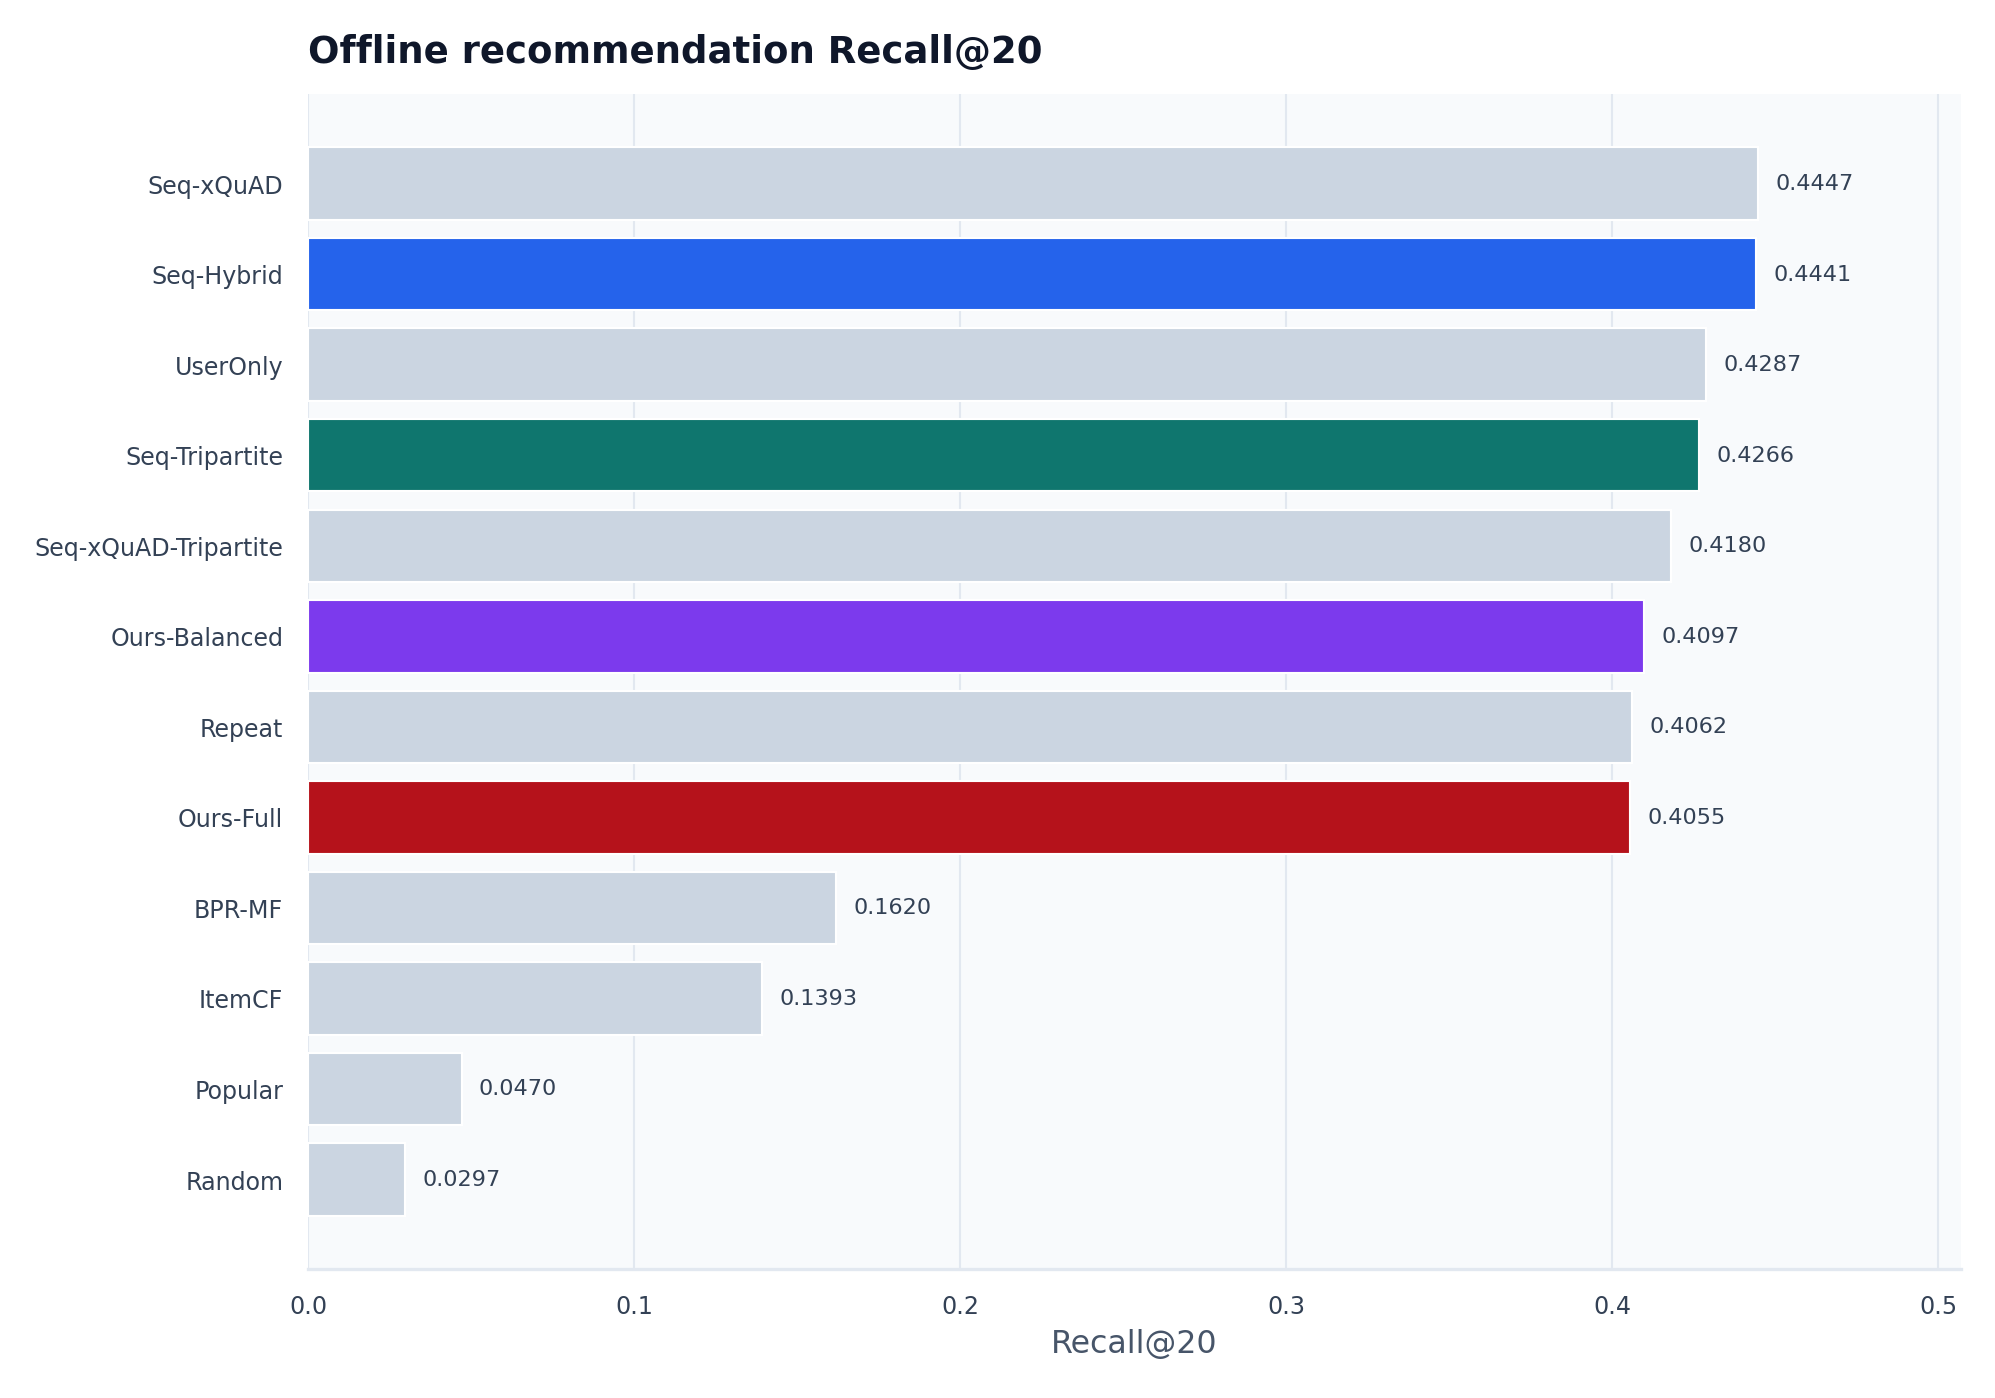
\includegraphics[width=\linewidth]{../../outputs/figures/offline_recall20.png}
            \caption{各模型 Recall@20 对比}
            \label{fig:recall20}
        \end{subfigure}
        \hfill
        \begin{subfigure}{0.48\linewidth}
            \centering
            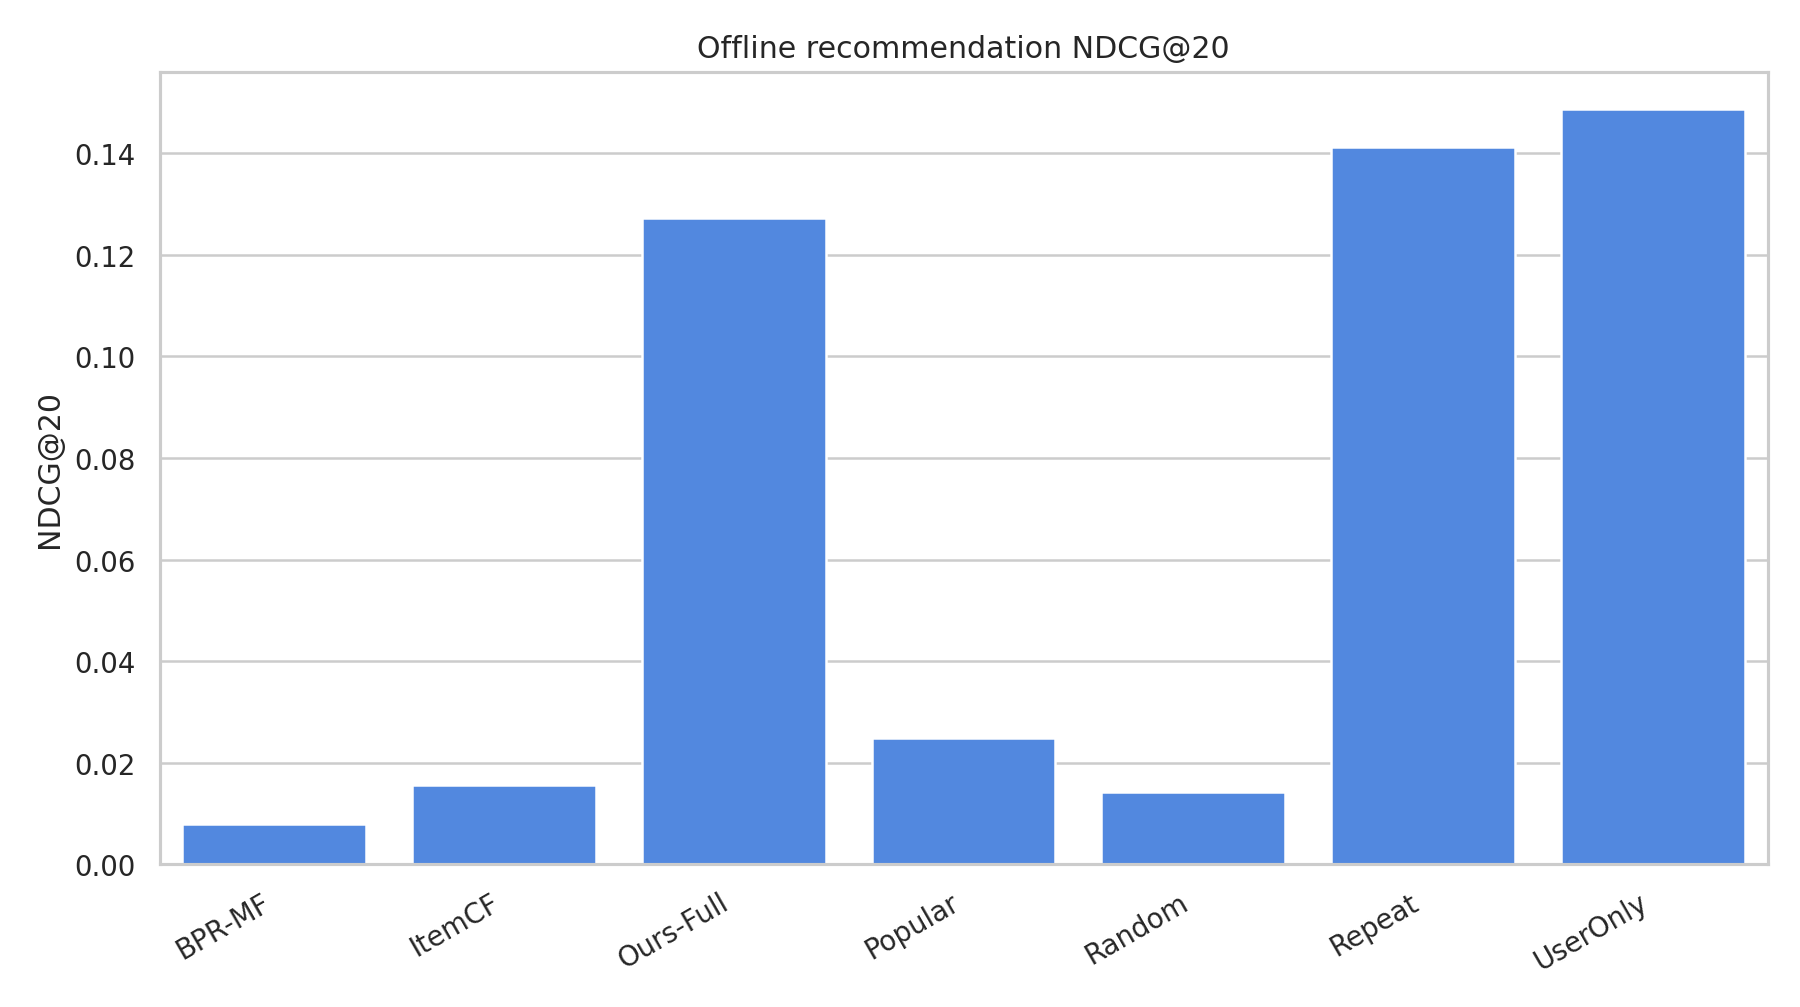
\includegraphics[width=\linewidth]{../../outputs/figures/offline_ndcg20.png}
            \caption{各模型 NDCG@20 对比}
            \label{fig:ndcg20}
        \end{subfigure}
        \caption{离线推荐准确率指标对比}
        \label{fig:offline_acc}
    \end{figure}

    \begin{figure}[htbp]
        \centering
        \begin{subfigure}{0.48\linewidth}
            \centering
            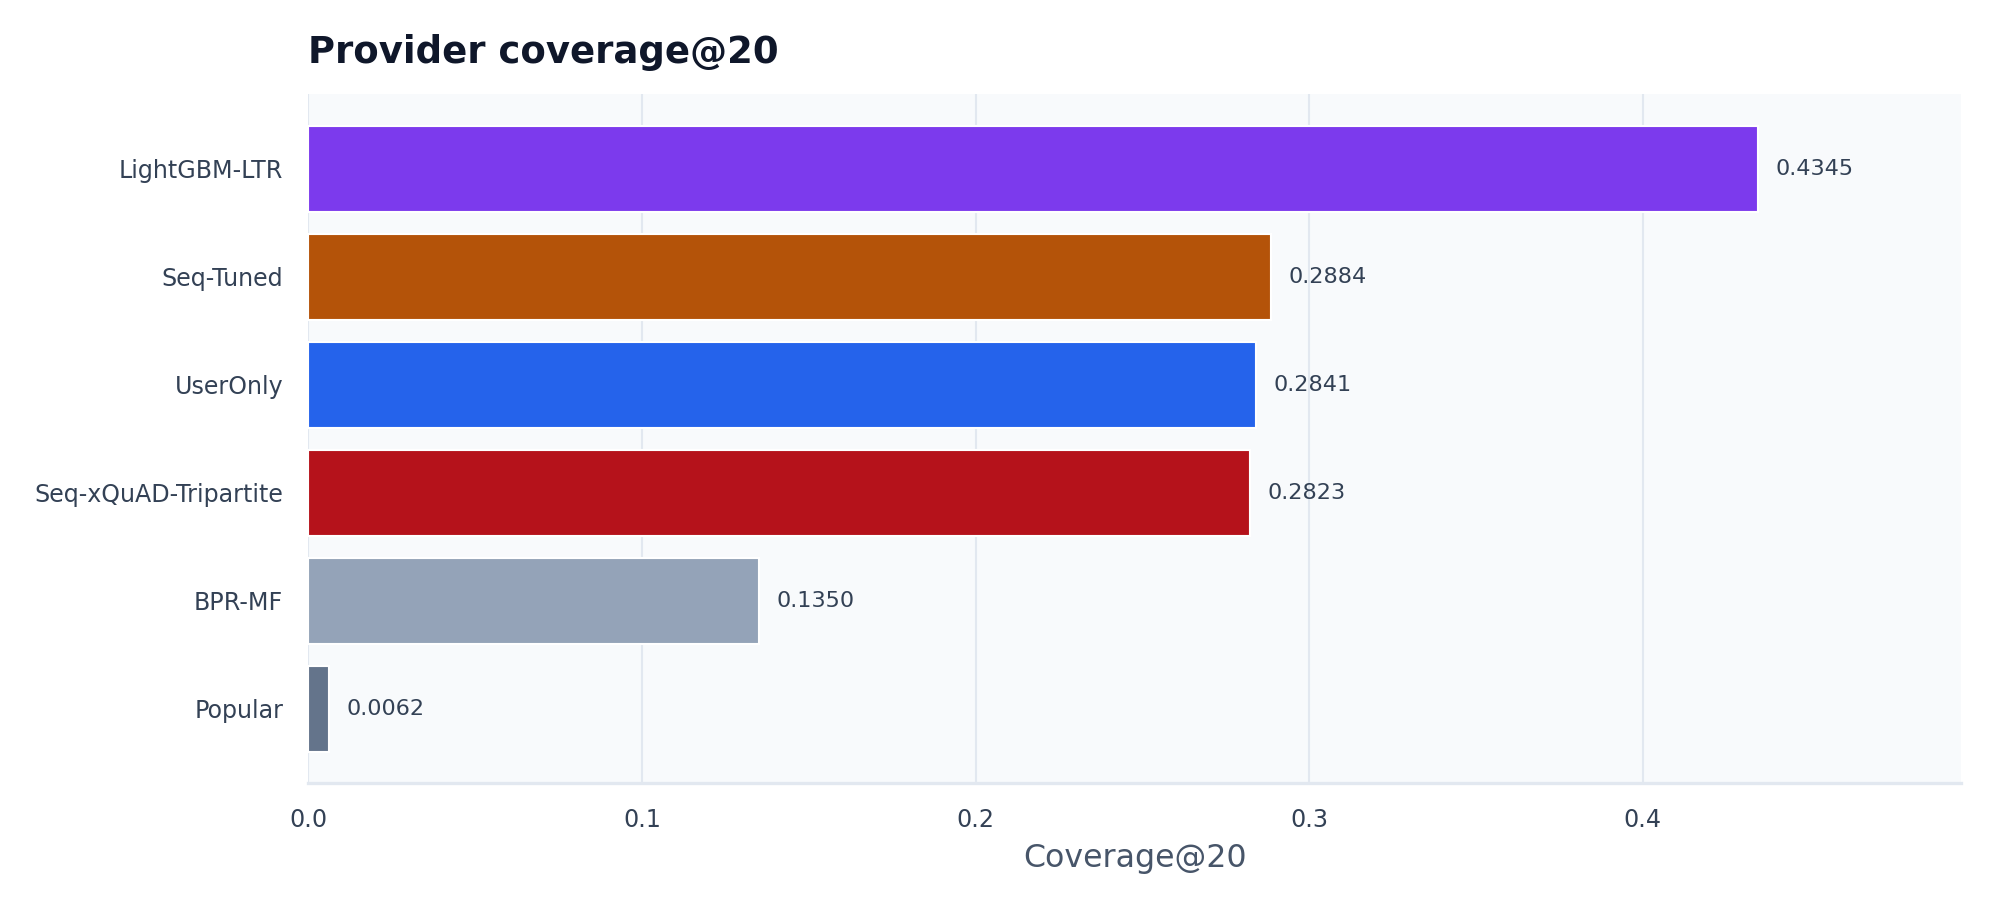
\includegraphics[width=\linewidth]{../../outputs/figures/offline_coverage20.png}
            \caption{各模型 Coverage@20 对比}
            \label{fig:coverage20}
        \end{subfigure}
        \hfill
        \begin{subfigure}{0.48\linewidth}
            \centering
            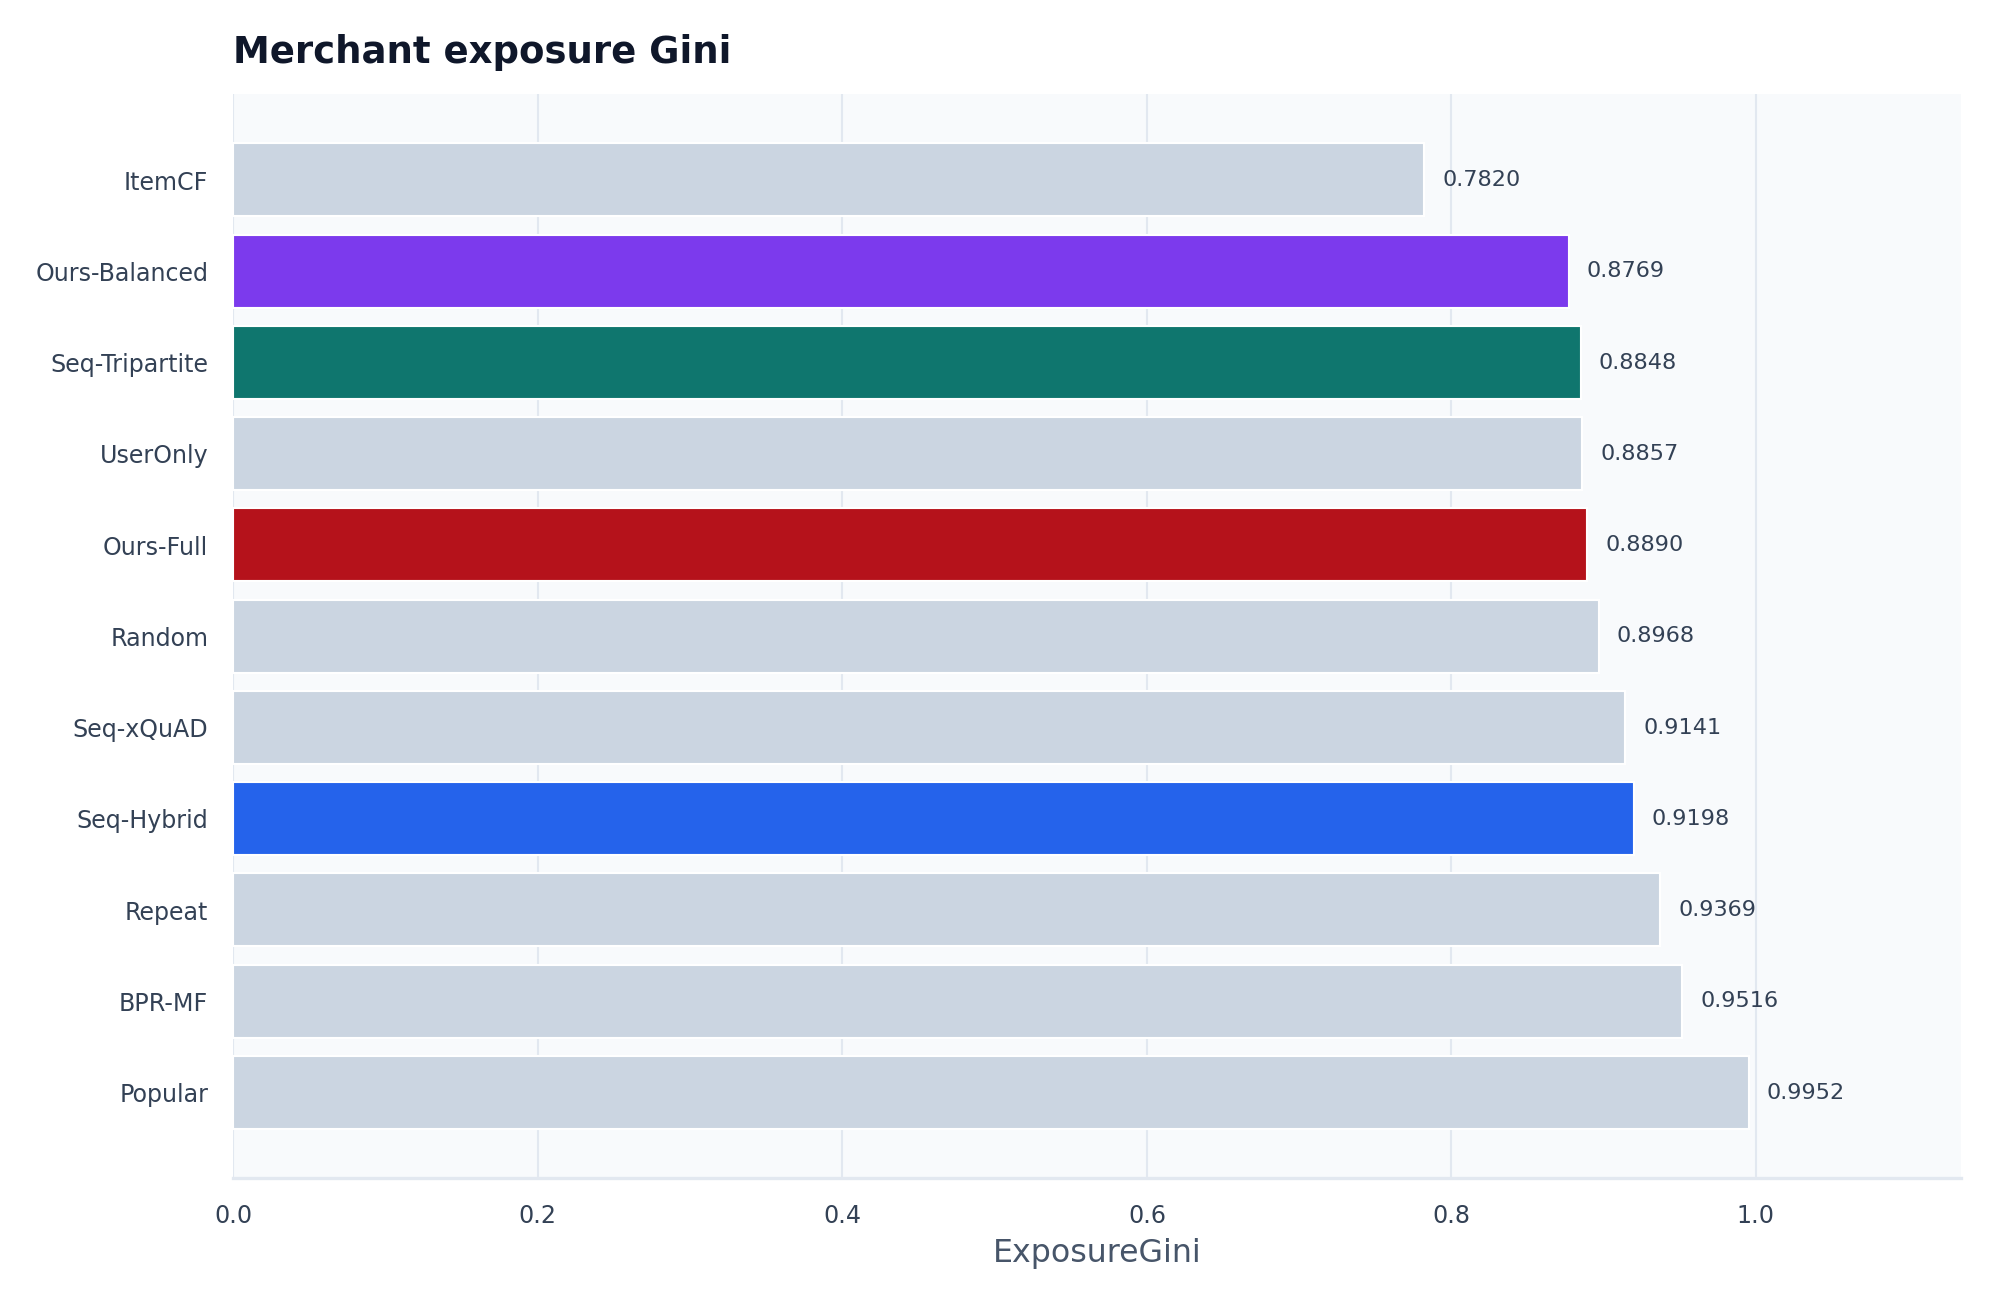
\includegraphics[width=\linewidth]{../../outputs/figures/offline_exposure_gini.png}
            \caption{各模型 Exposure Gini 对比}
            \label{fig:gini}
        \end{subfigure}
        \caption{商家侧指标对比}
        \label{fig:offline_merchant}
    \end{figure}

    从图 \ref{fig:offline_acc} 可以直观看出，Seq-Tuned 和 LightGBM-LTR 在 Recall 和 NDCG 上明显领先于其他模型。图 \ref{fig:offline_merchant} 则展示了商家侧指标：LightGBM-LTR 的 Coverage 最高、Exposure Gini 最低，体现了学习排序在突破"热度偏差"方面的优势。

    图 \ref{fig:category_jsd} 展示了 CategoryJSD@20 指标——衡量推荐列表品类分布与用户历史品类分布的 Jensen-Shannon 散度。Seq-Tuned 和 UserOnly 在该指标上表现最优，数值越低说明推荐品类越贴近用户真实消费习惯。

    \begin{figure}[htbp]
        \centering
        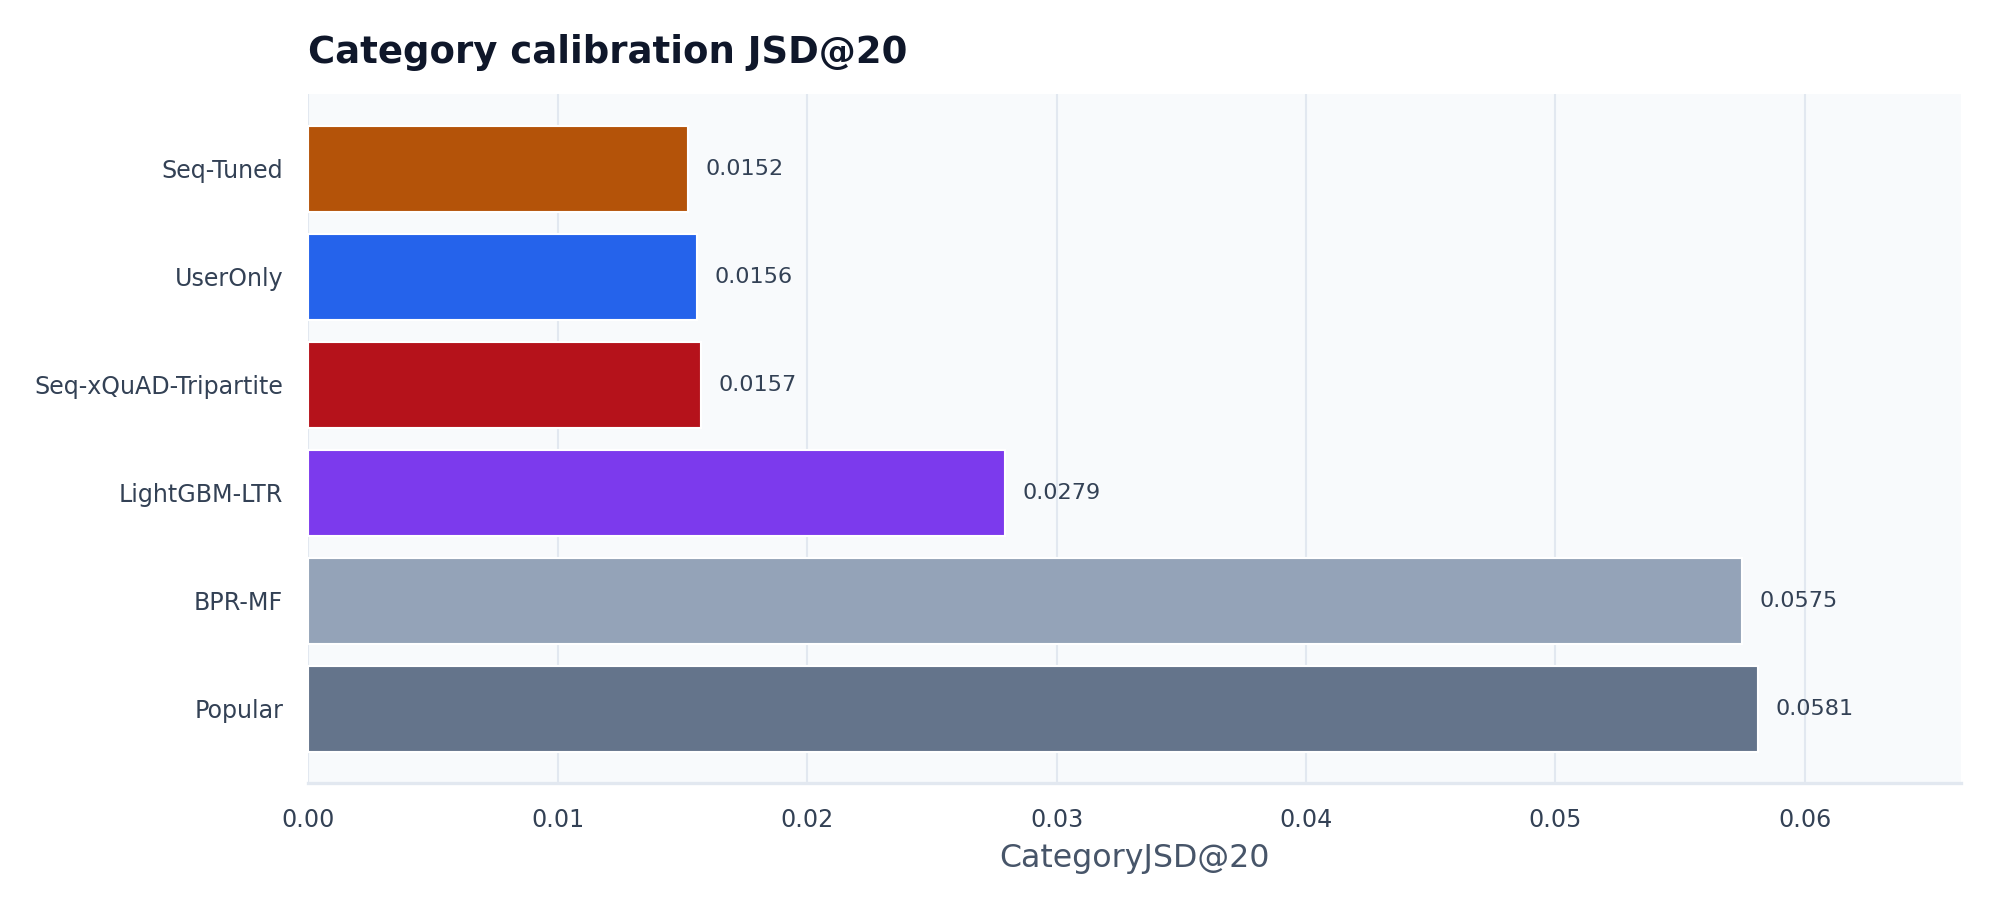
\includegraphics[width=0.65\linewidth]{../../outputs/figures/offline_category_jsd20.png}
        \caption{各模型 CategoryJSD@20 对比}
        \label{fig:category_jsd}
    \end{figure}

    \subsection{权衡分析：准确率 vs 公平性}

    推荐系统的核心挑战在于准确率与公平性之间的权衡。图 \ref{fig:tradeoff_ndcg_gini} 以 NDCG@20 为纵轴、Exposure Gini 为横轴，展示各模型在准确率-公平性二维空间中的位置。

    \begin{figure}[htbp]
        \centering
        \begin{subfigure}{0.48\linewidth}
            \centering
            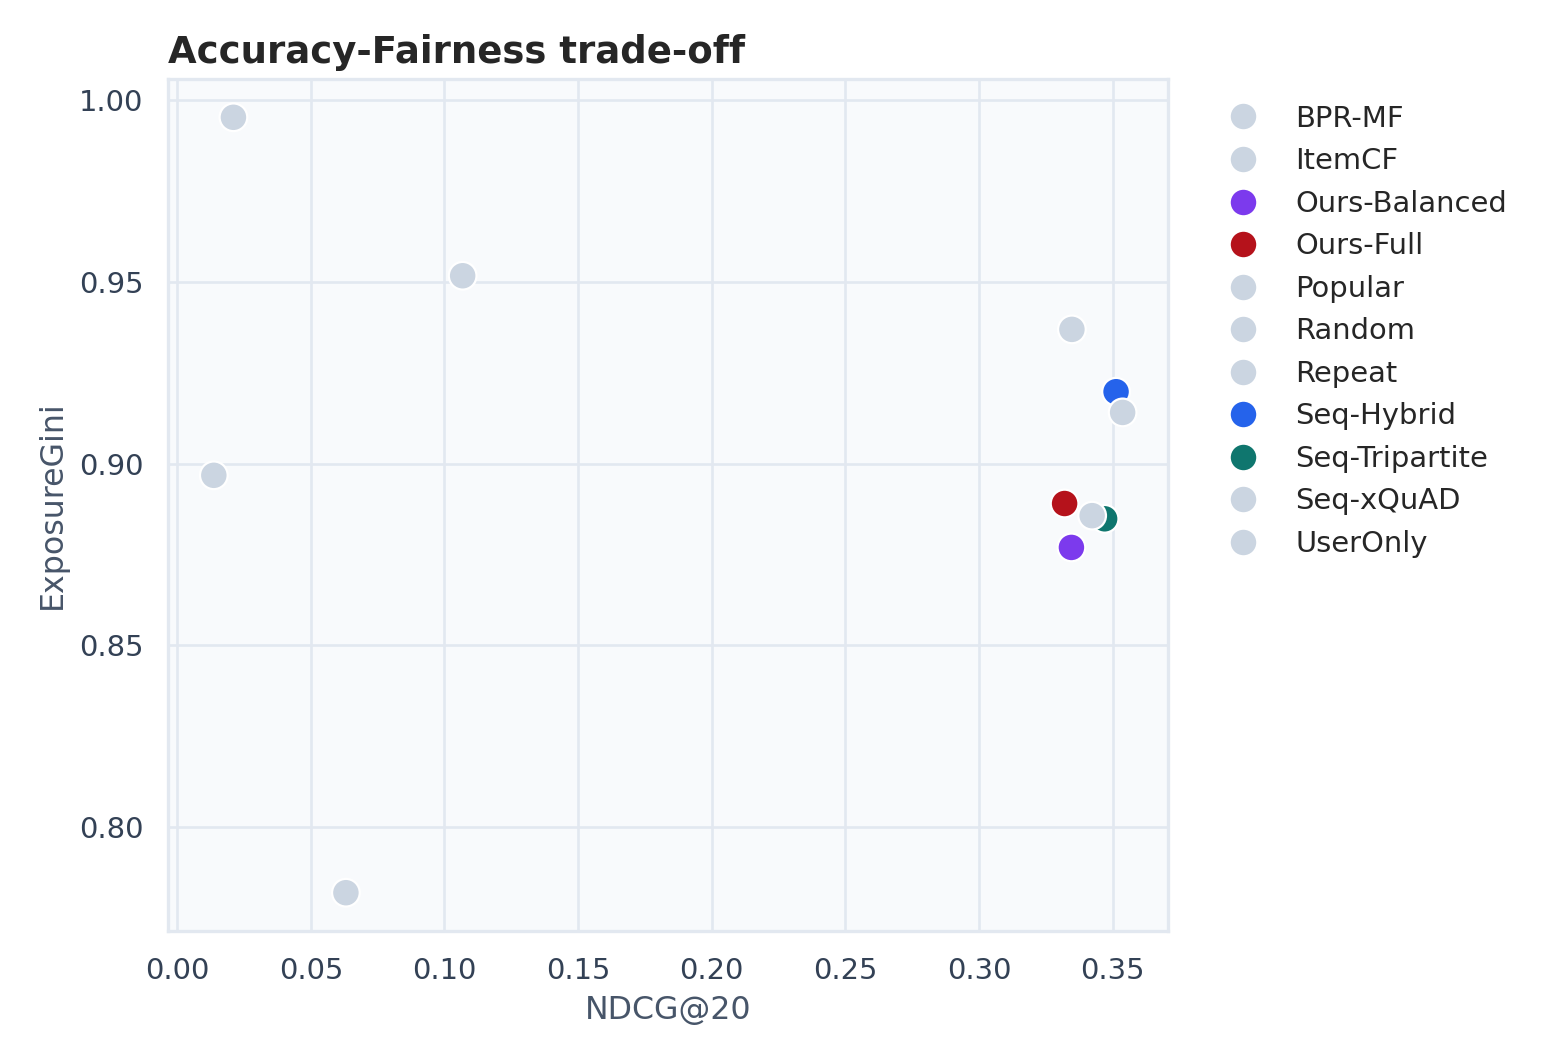
\includegraphics[width=\linewidth]{../../outputs/figures/tradeoff_ndcg_gini.png}
            \caption{NDCG@20 与 Exposure Gini 的权衡}
            \label{fig:tradeoff_ndcg_gini}
        \end{subfigure}
        \hfill
        \begin{subfigure}{0.48\linewidth}
            \centering
            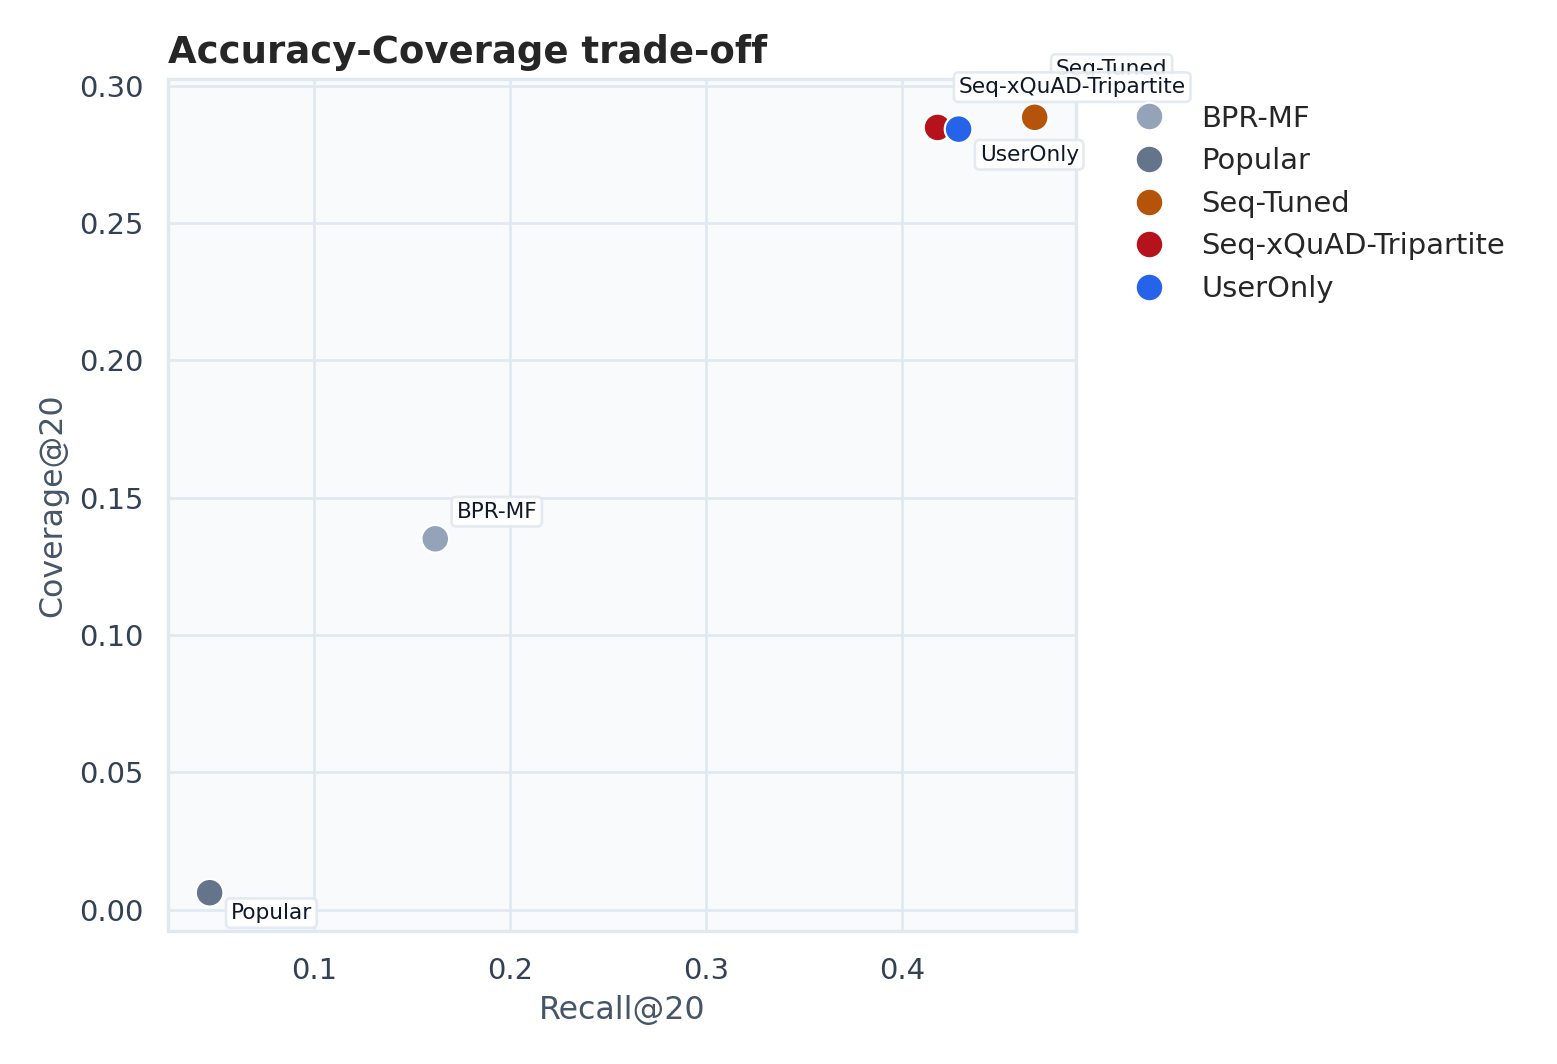
\includegraphics[width=\linewidth]{../../outputs/figures/tradeoff_recall_coverage.png}
            \caption{Recall@20 与 Coverage@20 的权衡}
            \label{fig:tradeoff_recall_coverage}
        \end{subfigure}
        \caption{准确率与公平性/覆盖面的权衡分析}
        \label{fig:tradeoff}
    \end{figure}

    从图 \ref{fig:tradeoff} 可以看到，LightGBM-LTR 位于准确率-公平性前沿的右下角（高准确率、低曝光集中度），Seq-Tuned 则位于高准确率但曝光略集中的位置，三方模型在保持较高准确率的同时维持了适中的公平性。

    \subsection{动态履约仿真结果（常规运力）}

    仿真采用 10 个随机种子重复运行，报告均值与 95\% 置信区间。常规运力场景使用 120 名合成骑手、8 个时间步 $\times$ 每步 16 个请求 = 128 个请求/策略，Top-K = 10，MNL/Softmax 用户选择。主要策略链路的完整指标如表 \ref{tab:simulation} 所示。

    \begin{table}[htbp]
        \centering
        \caption{动态履约仿真完整指标（常规运力 120 骑手，10 种子均值 $\pm$ 95\% CI）}
        \label{tab:simulation}
        \footnotesize
        \begin{tabular}{lcccc}
            \toprule
            \textbf{策略} & \textbf{平均ETA} & \textbf{超时率} & \textbf{准时率} & \textbf{平台效用} \\
            \midrule
            Popular + Nearest & 59.06 $\pm$2.28 & 0.579 $\pm$0.023 & 0.421 $\pm$0.023 & 0.391 $\pm$0.007 \\
            UserOnly + MinETA & 41.54 $\pm$1.23 & 0.347 $\pm$0.031 & 0.653 $\pm$0.031 & 0.511 $\pm$0.009 \\
            Seq-Tuned + MinETA & 40.44 $\pm$1.21 & 0.287 $\pm$0.041 & 0.713 $\pm$0.041 & 0.533 $\pm$0.012 \\
            LightGBM-LTR + MinETA & 40.45 $\pm$1.11 & 0.299 $\pm$0.028 & 0.701 $\pm$0.028 & 0.528 $\pm$0.011 \\
            Seq-xQuAD-Tripartite + Greedy & 37.04 $\pm$1.91 & 0.212 $\pm$0.046 & 0.788 $\pm$0.046 & 0.550 $\pm$0.012 \\
            Seq-xQuAD-Tripartite + Batch & 35.90 $\pm$1.88 & 0.195 $\pm$0.036 & 0.805 $\pm$0.036 & 0.553 $\pm$0.009 \\
            Session-SPU-Tripartite + Greedy & 38.14 $\pm$1.35 & 0.220 $\pm$0.031 & 0.780 $\pm$0.031 & 0.557 $\pm$0.011 \\
            \textbf{Session-SPU-Tripartite + Batch} & 36.79 $\pm$1.25 & 0.199 $\pm$0.029 & 0.801 $\pm$0.029 & \textbf{0.557} $\pm$0.010 \\
            KG-Tripartite + Batch & 36.90 $\pm$1.04 & 0.211 $\pm$0.033 & 0.789 $\pm$0.033 & 0.550 $\pm$0.011 \\
            KG-Tripartite + RouteMinETA & 36.15 $\pm$0.96 & 0.229 $\pm$0.037 & 0.771 $\pm$0.037 & 0.542 $\pm$0.011 \\
            KG-Tripartite + RouteBatch & 38.84 $\pm$1.24 & 0.311 $\pm$0.049 & 0.689 $\pm$0.049 & 0.517 $\pm$0.014 \\
            \bottomrule
        \end{tabular}
    \end{table}

    从表 \ref{tab:simulation} 可以得出以下结论：

    \begin{enumerate}
        \item \textbf{三方方法在履约指标上全面优于纯用户侧方法。}Session-SPU-Tripartite + Batch 取得了最高的平台效用（0.557），Seq-xQuAD-Tripartite + Batch 取得了最低的平均 ETA（35.90 分钟）和最低的超时率（0.195）。
        \item \textbf{批量二分图匹配优于贪心逐单分配。}Seq-xQuAD-Tripartite 下，Batch 模式的超时率（0.195）低于 Greedy 模式（0.212），说明全局最优匹配能有效平衡骑手负载。
        \item \textbf{KG-Tripartite 在常规运力下与最优策略统计打平。}KG-Tripartite + Batch 的平均 ETA（36.90）和平台效用（0.550）与 Session-SPU-Tripartite 的置信区间重叠，表明图谱信号与 Session/SPU 信号在推荐-履约链路中具有互补性。
        \item \textbf{顺路派单在常规运力下 ETA 与槽位匹配打平。}KG-Tripartite + RouteMinETA 的平均 ETA（36.15）与 Batch 最优值（35.90）的置信区间重叠——骑手大多空闲时，分散派单即是最优解，合单不会带来额外收益；且 route 家族的 ETA 诚实计入队列沿路径行进的时间，口径更严格。
        \item \textbf{离线准确率最优不等于仿真效果最优。}Seq-Tuned 在离线 Recall 上最高，但在仿真中超时率（0.287）高于三方方法，说明纯粹追求准确率的推荐可能将订单引导至配送压力大的商家。
    \end{enumerate}

    \subsection{运力紧张压力场景}

    为验证顺路派单在高峰爆单场景下的价值，使用 30 名骑手（常规运力的 25\%）模拟运力紧张的压力场景。10 种子均值结果如表 \ref{tab:sim_stress} 所示。

    \begin{table}[htbp]
        \centering
        \caption{运力紧张压力场景仿真（30 骑手，10 种子均值 $\pm$ 95\% CI）}
        \label{tab:sim_stress}
        \footnotesize
        \begin{tabular}{lcccc}
            \toprule
            \textbf{策略} & \textbf{平均ETA} & \textbf{超时率} & \textbf{平台效用} & \textbf{顺路接单率} \\
            \midrule
            Popular + Nearest & 76.86 $\pm$2.56 & 0.749 $\pm$0.029 & 0.412 $\pm$0.012 & --- \\
            Seq-Tuned + MinETA & 76.64 $\pm$2.46 & 0.819 $\pm$0.014 & 0.442 $\pm$0.014 & --- \\
            Seq-xQuAD-Tripartite + Batch & 60.96 $\pm$4.84 & 0.679 $\pm$0.046 & 0.486 $\pm$0.017 & --- \\
            KG-Tripartite + Batch & 61.47 $\pm$2.85 & 0.685 $\pm$0.039 & 0.481 $\pm$0.014 & --- \\
            \textbf{KG-Tripartite + RouteMinETA} & \textbf{44.88} $\pm$1.55 & \textbf{0.457} $\pm$0.038 & \textbf{0.544} $\pm$0.016 & 0.669 $\pm$0.016 \\
            KG-Tripartite + RouteBatch & 47.34 $\pm$1.66 & 0.515 $\pm$0.040 & 0.525 $\pm$0.015 & 0.666 $\pm$0.015 \\
            \bottomrule
        \end{tabular}
    \end{table}

    从表 \ref{tab:sim_stress} 可以得出：

    \begin{enumerate}
        \item \textbf{顺路派单在运力紧张时大幅反超。}KG-Tripartite + RouteMinETA 的平均 ETA（44.88 分钟）比最优槽位匹配（Seq-xQuAD-Tripartite + Batch，60.96 分钟）低约 16 分钟，远超置信区间范围；超时率从 0.679 降至 0.457。
        \item \textbf{顺路接单率达 66.9\%。}说明在运力吃紧时，cheapest-insertion 路径感知派单能有效利用骑手已有路径顺路接单，避免远距离单独调度。
        \item \textbf{无免费午餐。}顺路派单不是在所有场景下更优——运力充足时槽位批量匹配的 ETA 更好；顺路合单的优势出现在运力紧张的高峰场景。派单机制可随供需状态切换，这是三方联合视角的核心论据。
    \end{enumerate}

    \begin{figure}[htbp]
        \centering
        \begin{subfigure}{0.48\linewidth}
            \centering
            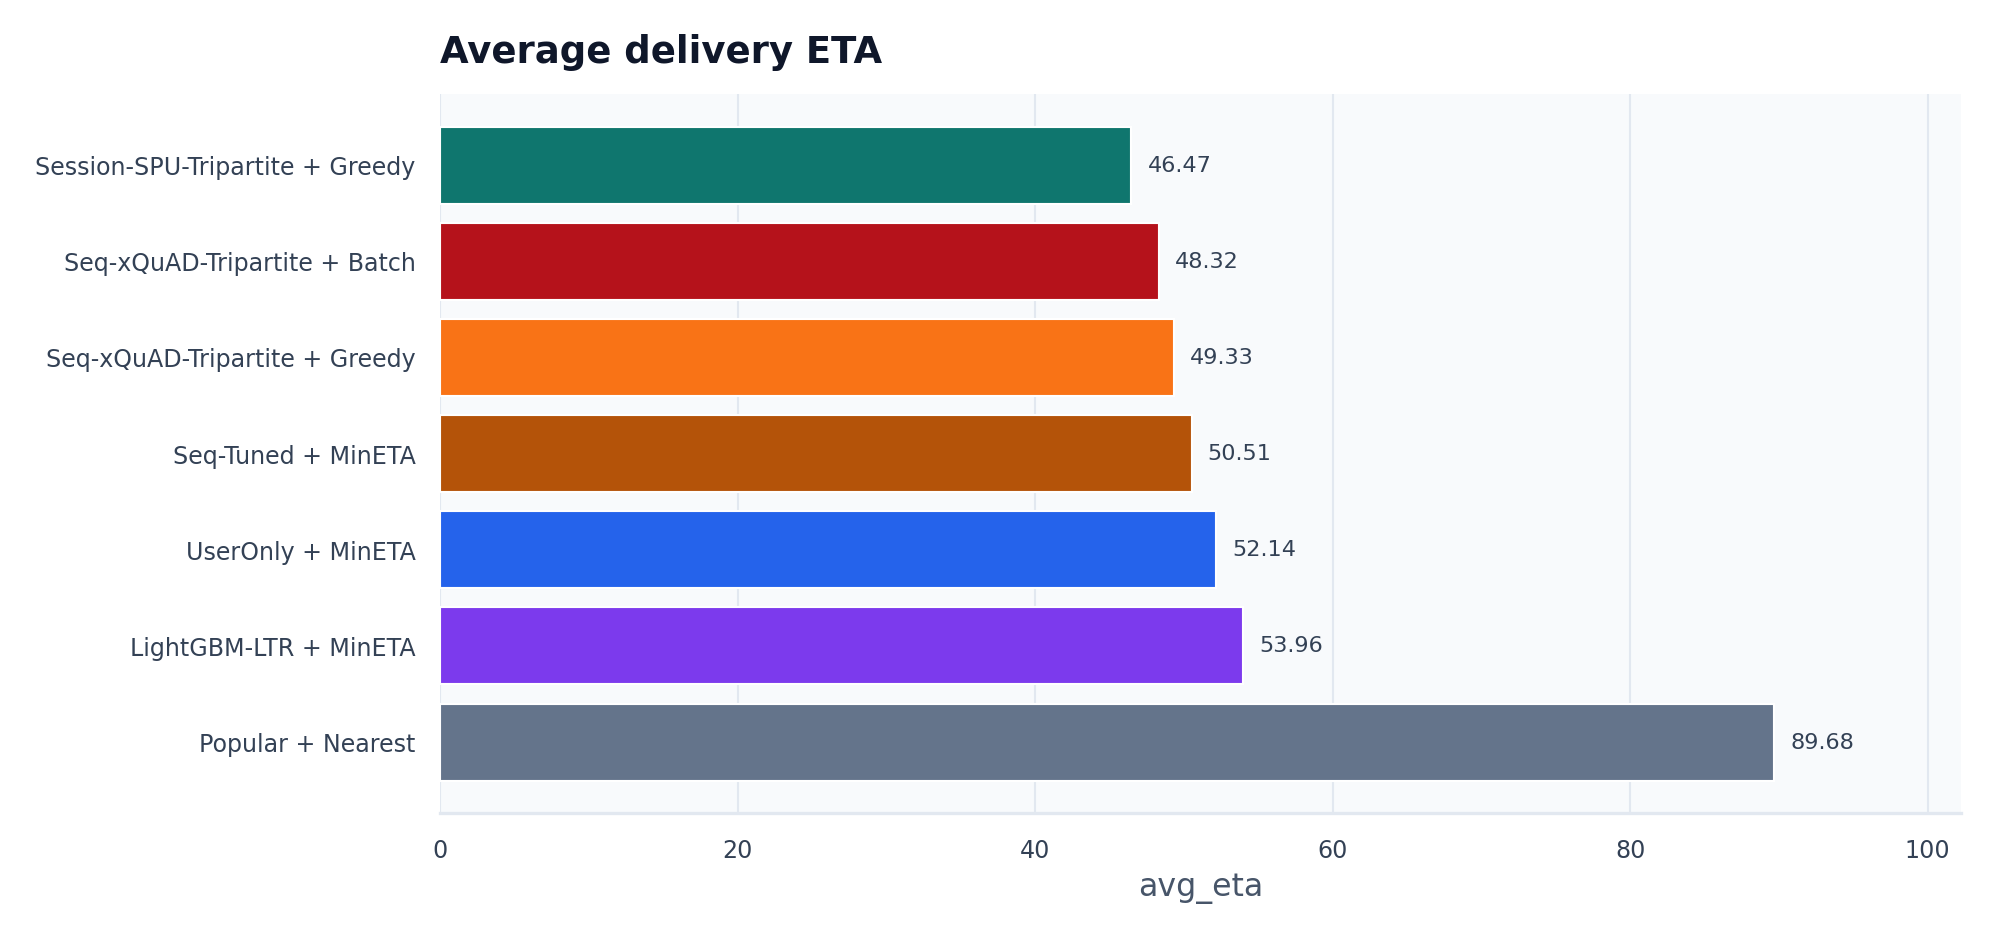
\includegraphics[width=\linewidth]{../../outputs/figures/simulation_avg_eta.png}
            \caption{各策略平均 ETA 对比}
            \label{fig:avg_eta}
        \end{subfigure}
        \hfill
        \begin{subfigure}{0.48\linewidth}
            \centering
            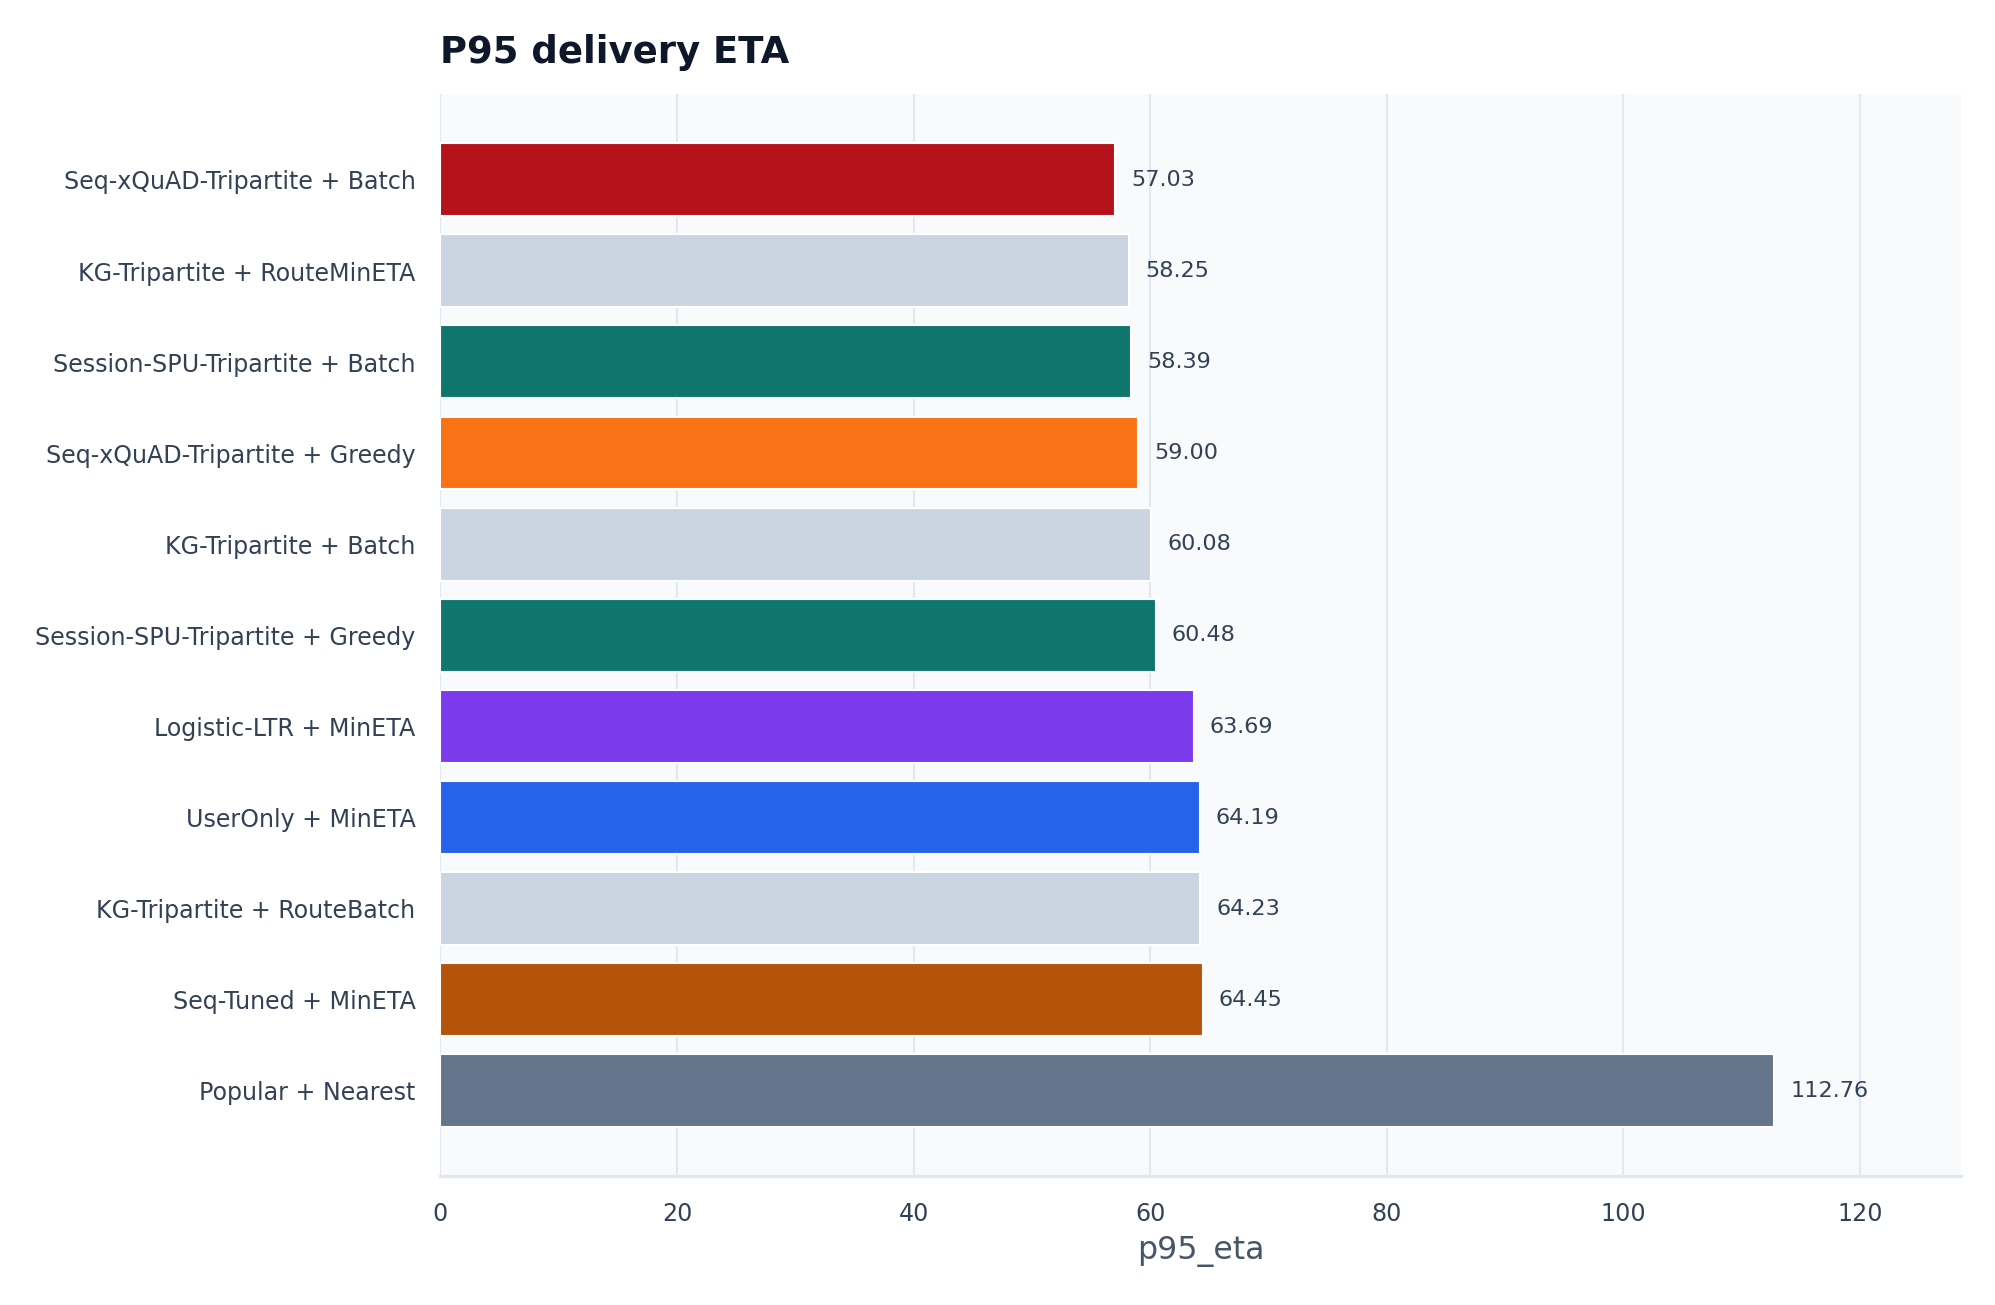
\includegraphics[width=\linewidth]{../../outputs/figures/simulation_p95_eta.png}
            \caption{各策略 P95 ETA 对比}
            \label{fig:p95_eta}
        \end{subfigure}
        \caption{配送时效指标对比}
        \label{fig:eta_metrics}
    \end{figure}

    \begin{figure}[htbp]
        \centering
        \begin{subfigure}{0.48\linewidth}
            \centering
            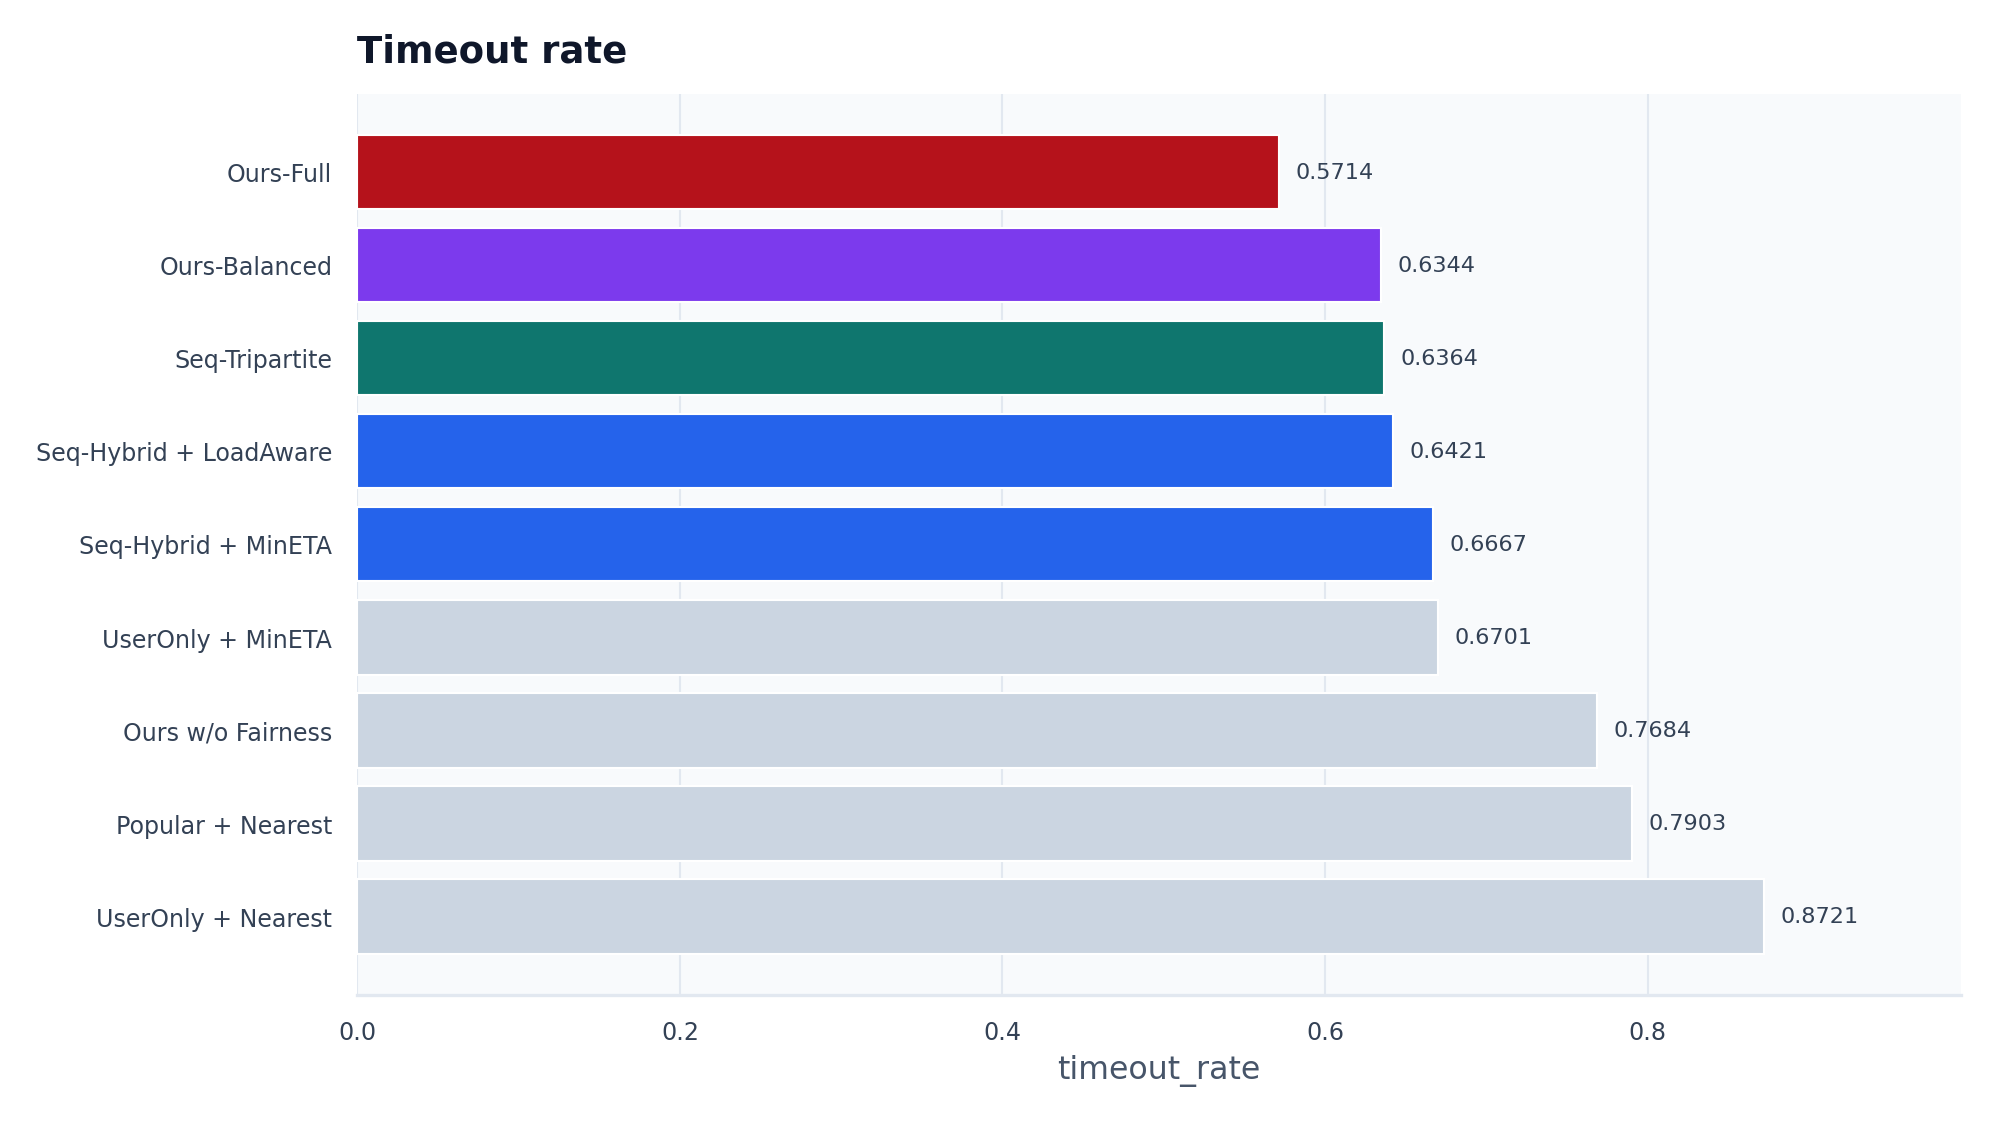
\includegraphics[width=\linewidth]{../../outputs/figures/simulation_timeout_rate.png}
            \caption{各策略超时率对比}
            \label{fig:timeout}
        \end{subfigure}
        \hfill
        \begin{subfigure}{0.48\linewidth}
            \centering
            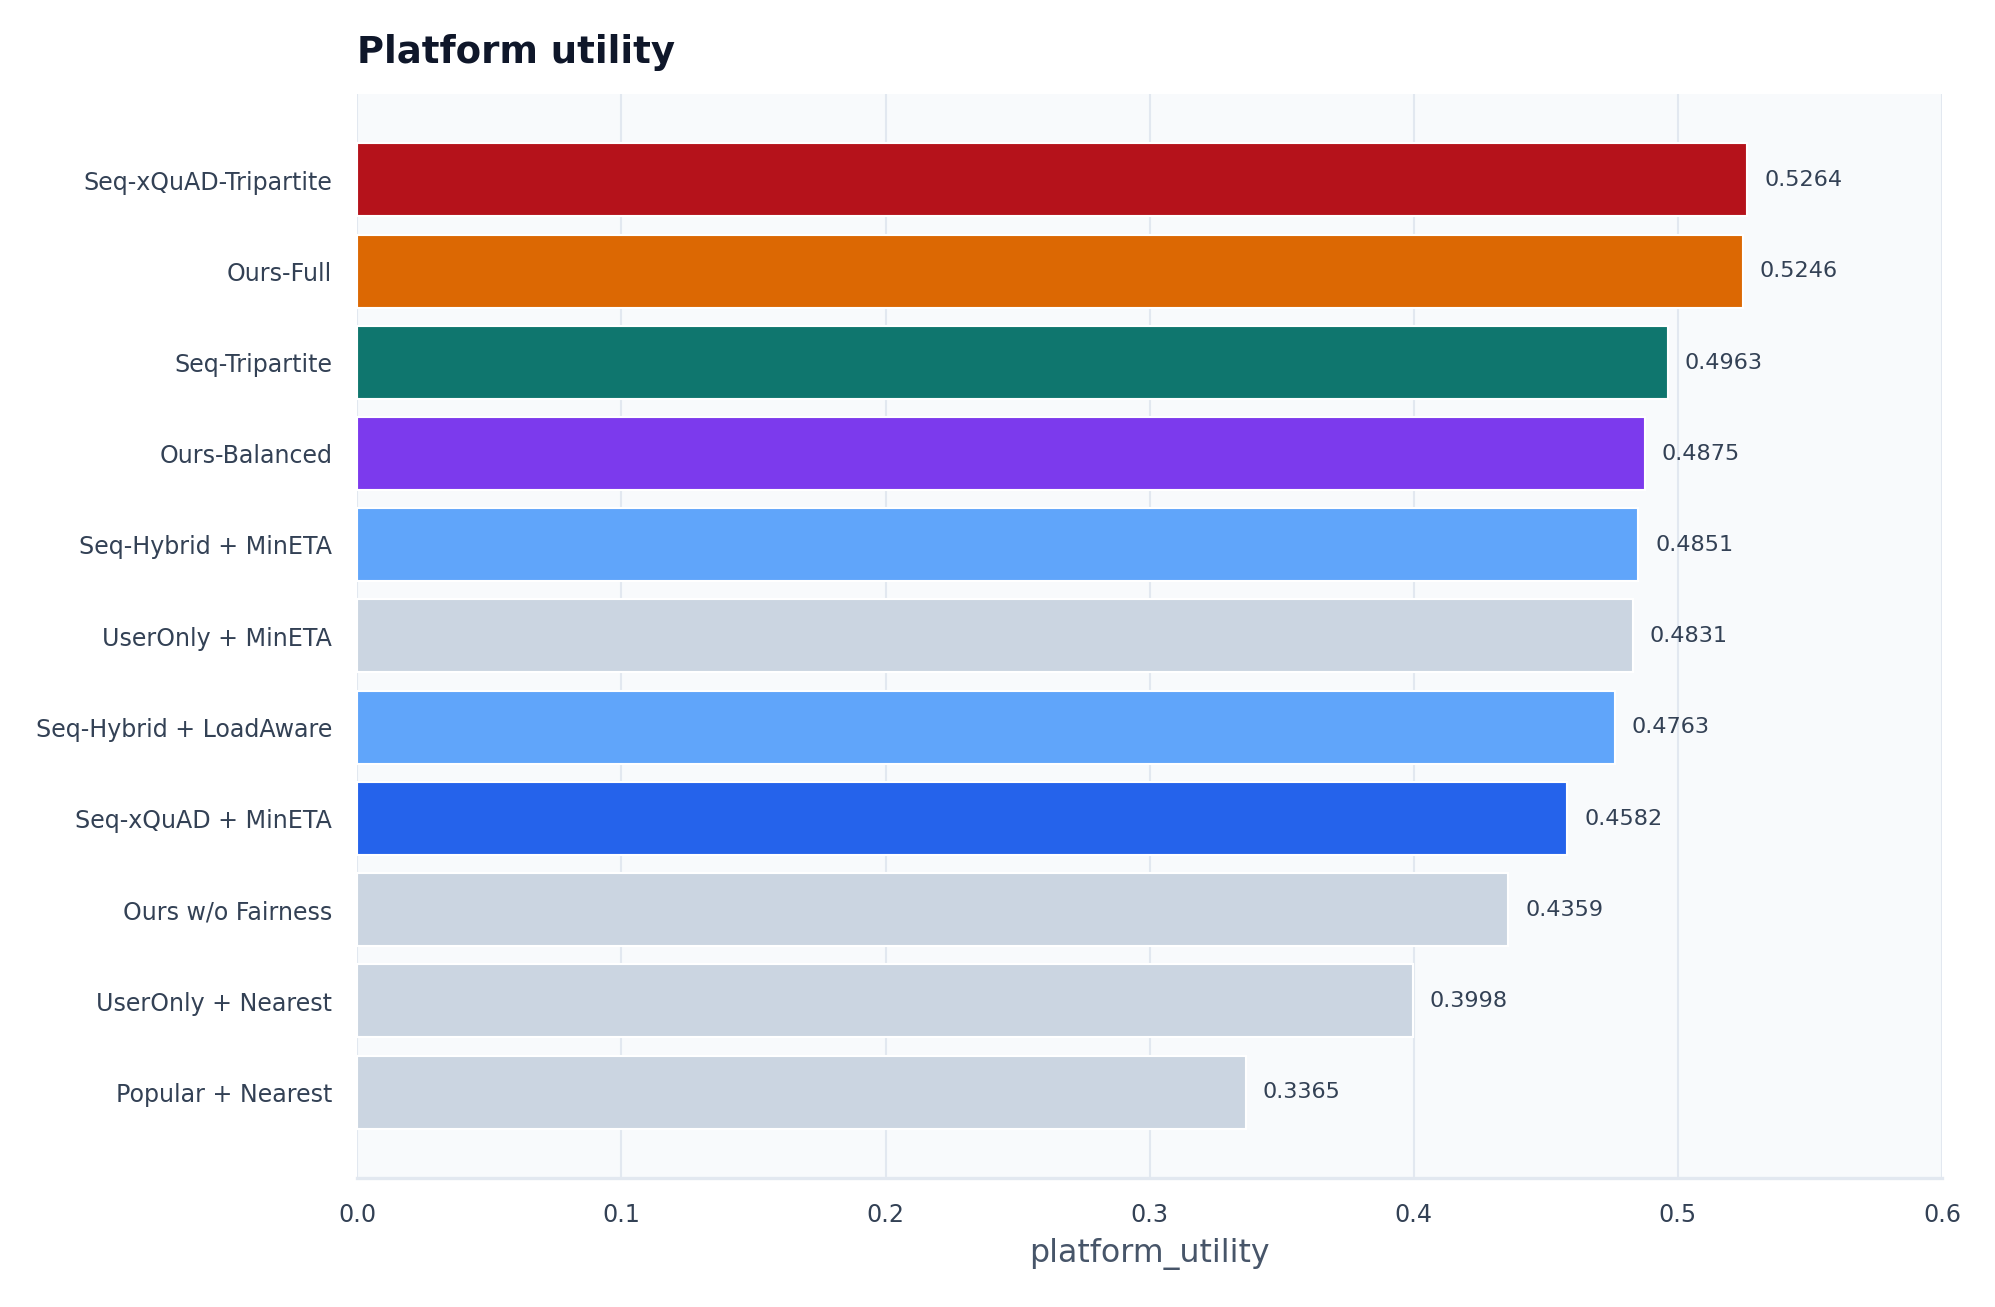
\includegraphics[width=\linewidth]{../../outputs/figures/simulation_platform_utility.png}
            \caption{各策略平台效用对比}
            \label{fig:platform_utility}
        \end{subfigure}
        \caption{履约质量与平台效用对比}
        \label{fig:sim_quality}
    \end{figure}

    从图 \ref{fig:eta_metrics} 和图 \ref{fig:sim_quality} 可以直观看到，三方策略（Seq-xQuAD-Tripartite、Session-SPU-Tripartite、KG-Tripartite）配合 Batch 匹配在平均 ETA、P95 ETA、超时率和平台效用上均显著优于纯用户侧策略。特别值得注意的是，从 Popular + Nearest 到 Seq-xQuAD-Tripartite + Batch，平台效用提升了约 41\%（从 0.391 到 0.553），平均 ETA 下降了约 39\%（从 59.06 分钟到 35.90 分钟）。

    \begin{figure}[htbp]
        \centering
        \begin{subfigure}{0.48\linewidth}
            \centering
            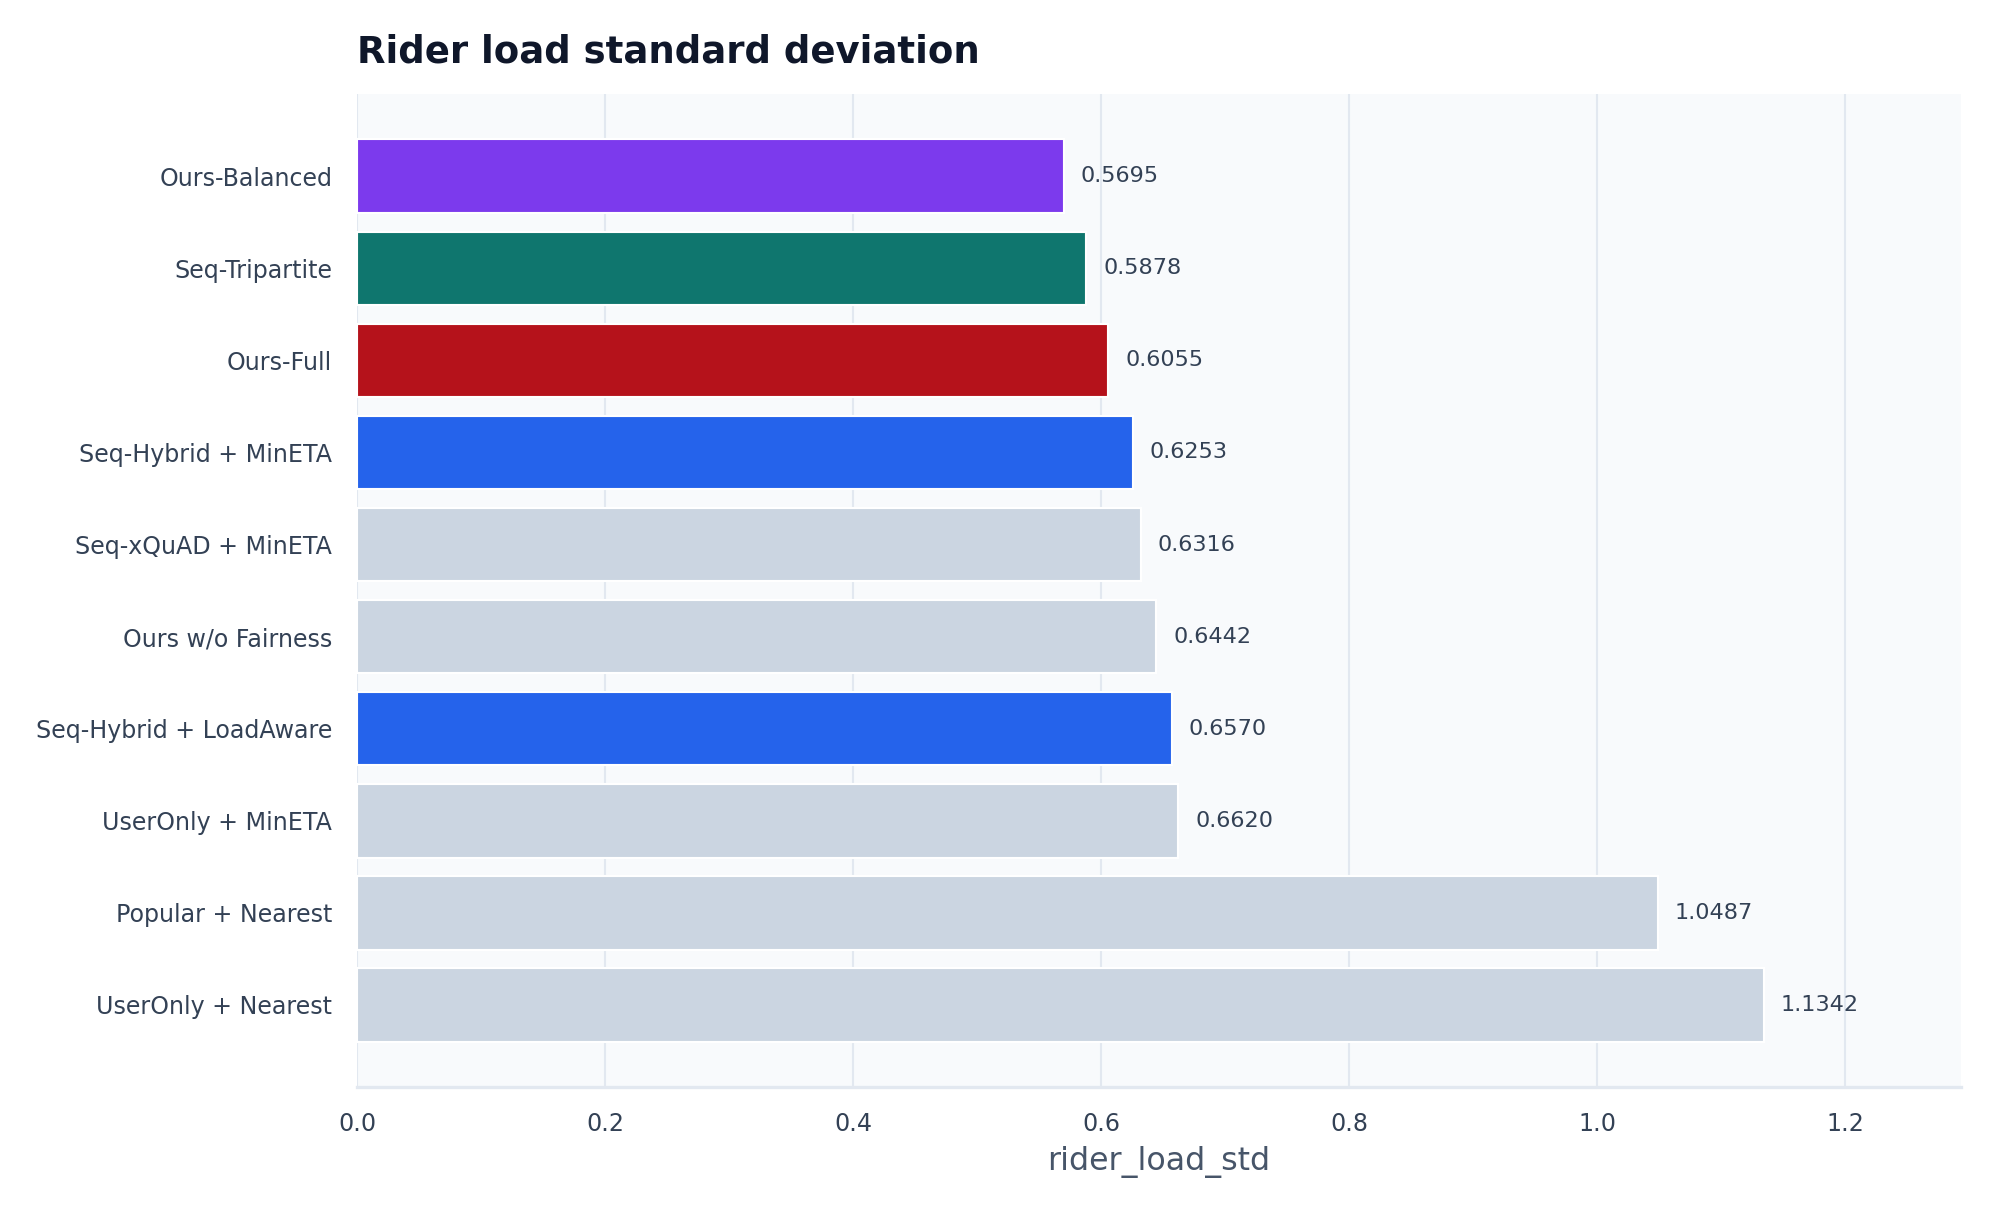
\includegraphics[width=\linewidth]{../../outputs/figures/simulation_rider_load_std.png}
            \caption{骑手负载标准差对比}
            \label{fig:rider_load}
        \end{subfigure}
        \hfill
        \begin{subfigure}{0.48\linewidth}
            \centering
            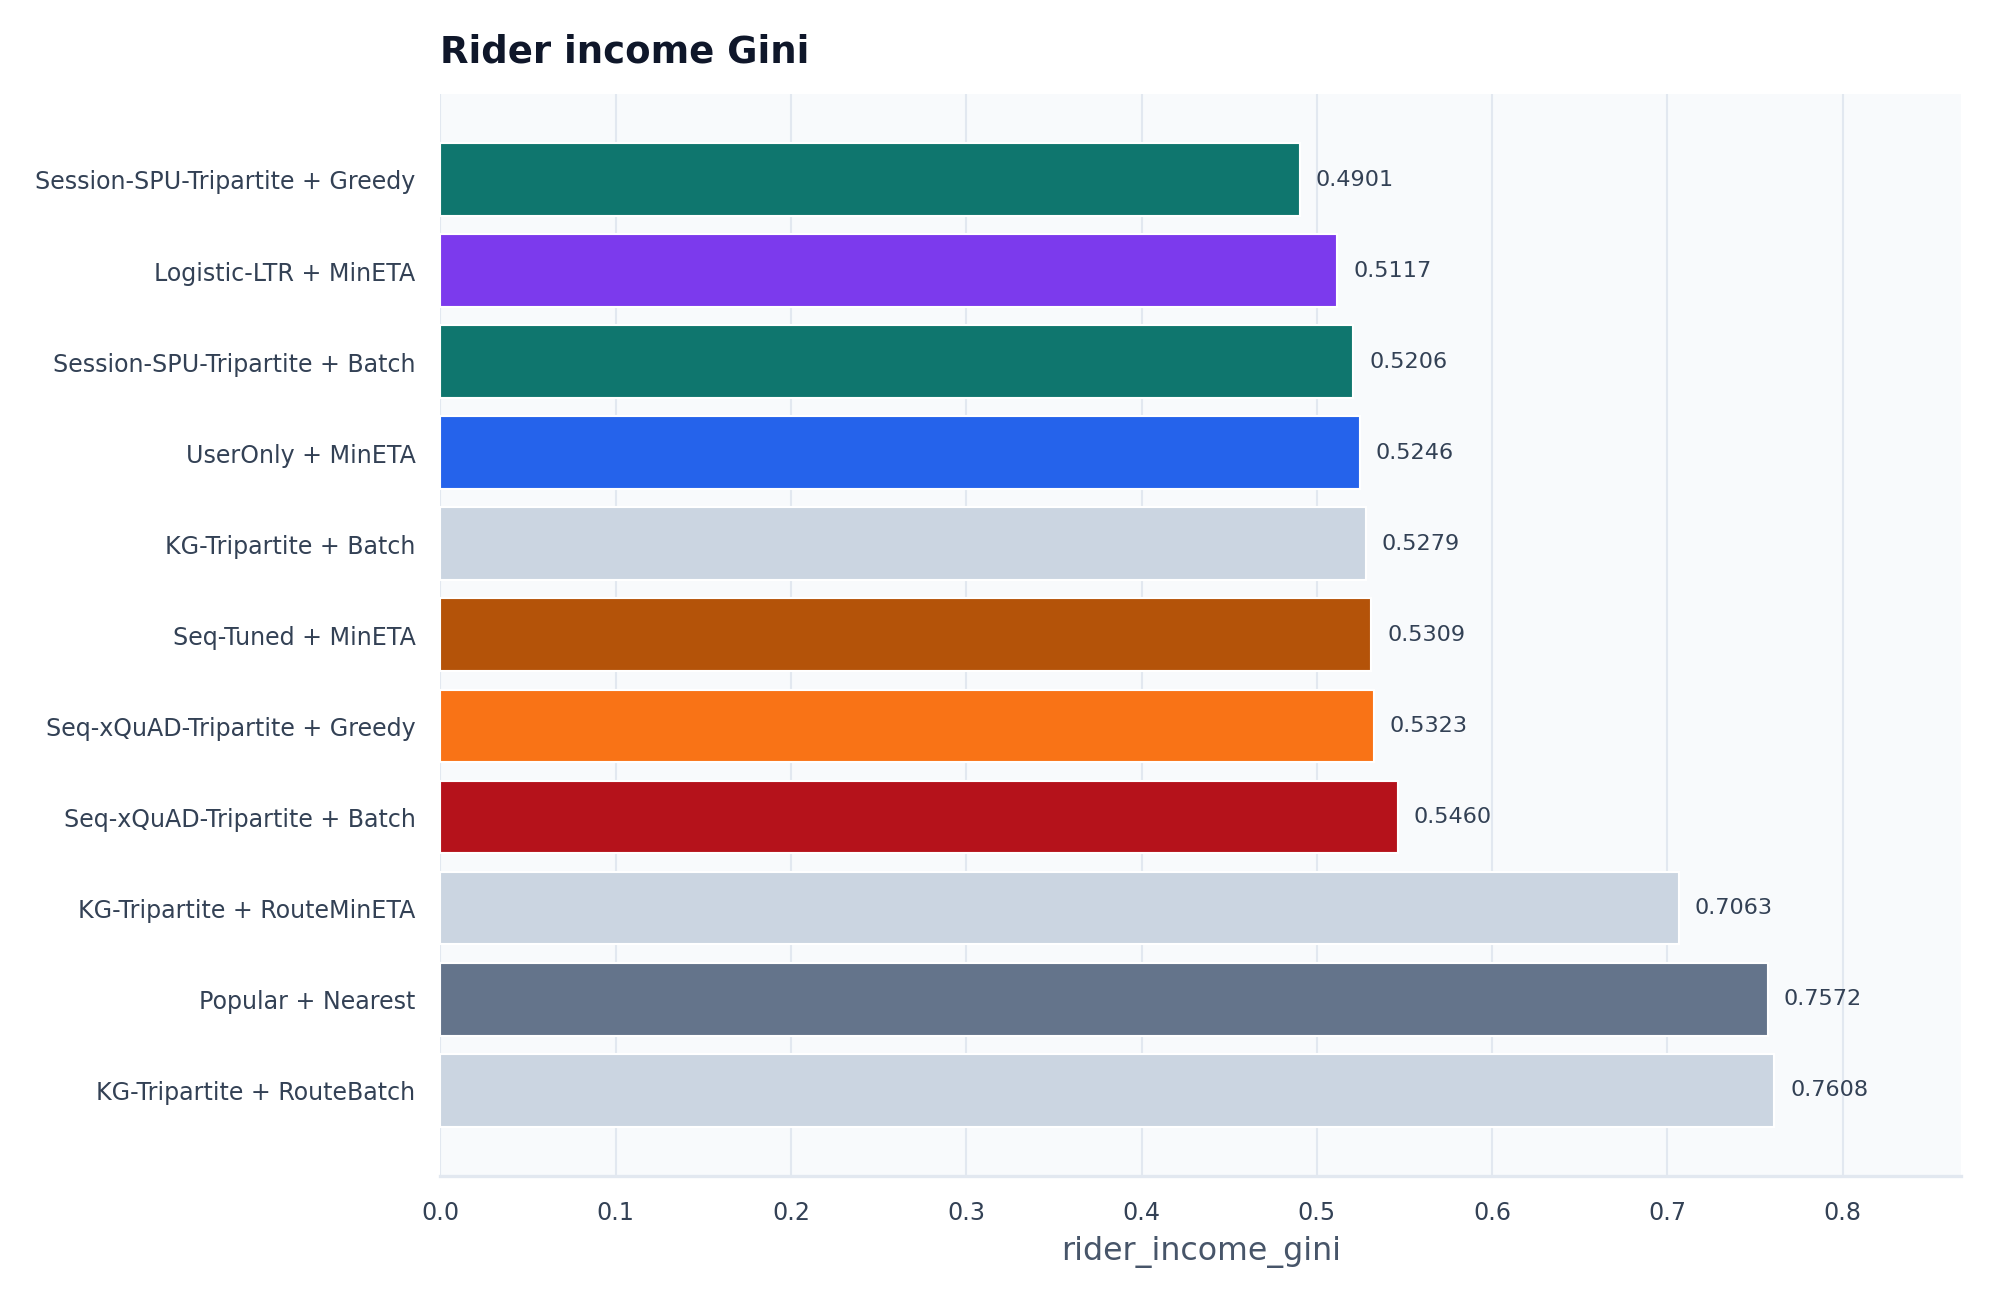
\includegraphics[width=\linewidth]{../../outputs/figures/simulation_rider_income_gini.png}
            \caption{骑手收入 Gini 对比}
            \label{fig:income_gini}
        \end{subfigure}
        \caption{骑手侧指标对比}
        \label{fig:rider_metrics}
    \end{figure}

    \begin{figure}[htbp]
        \centering
        \begin{subfigure}{0.48\linewidth}
            \centering
            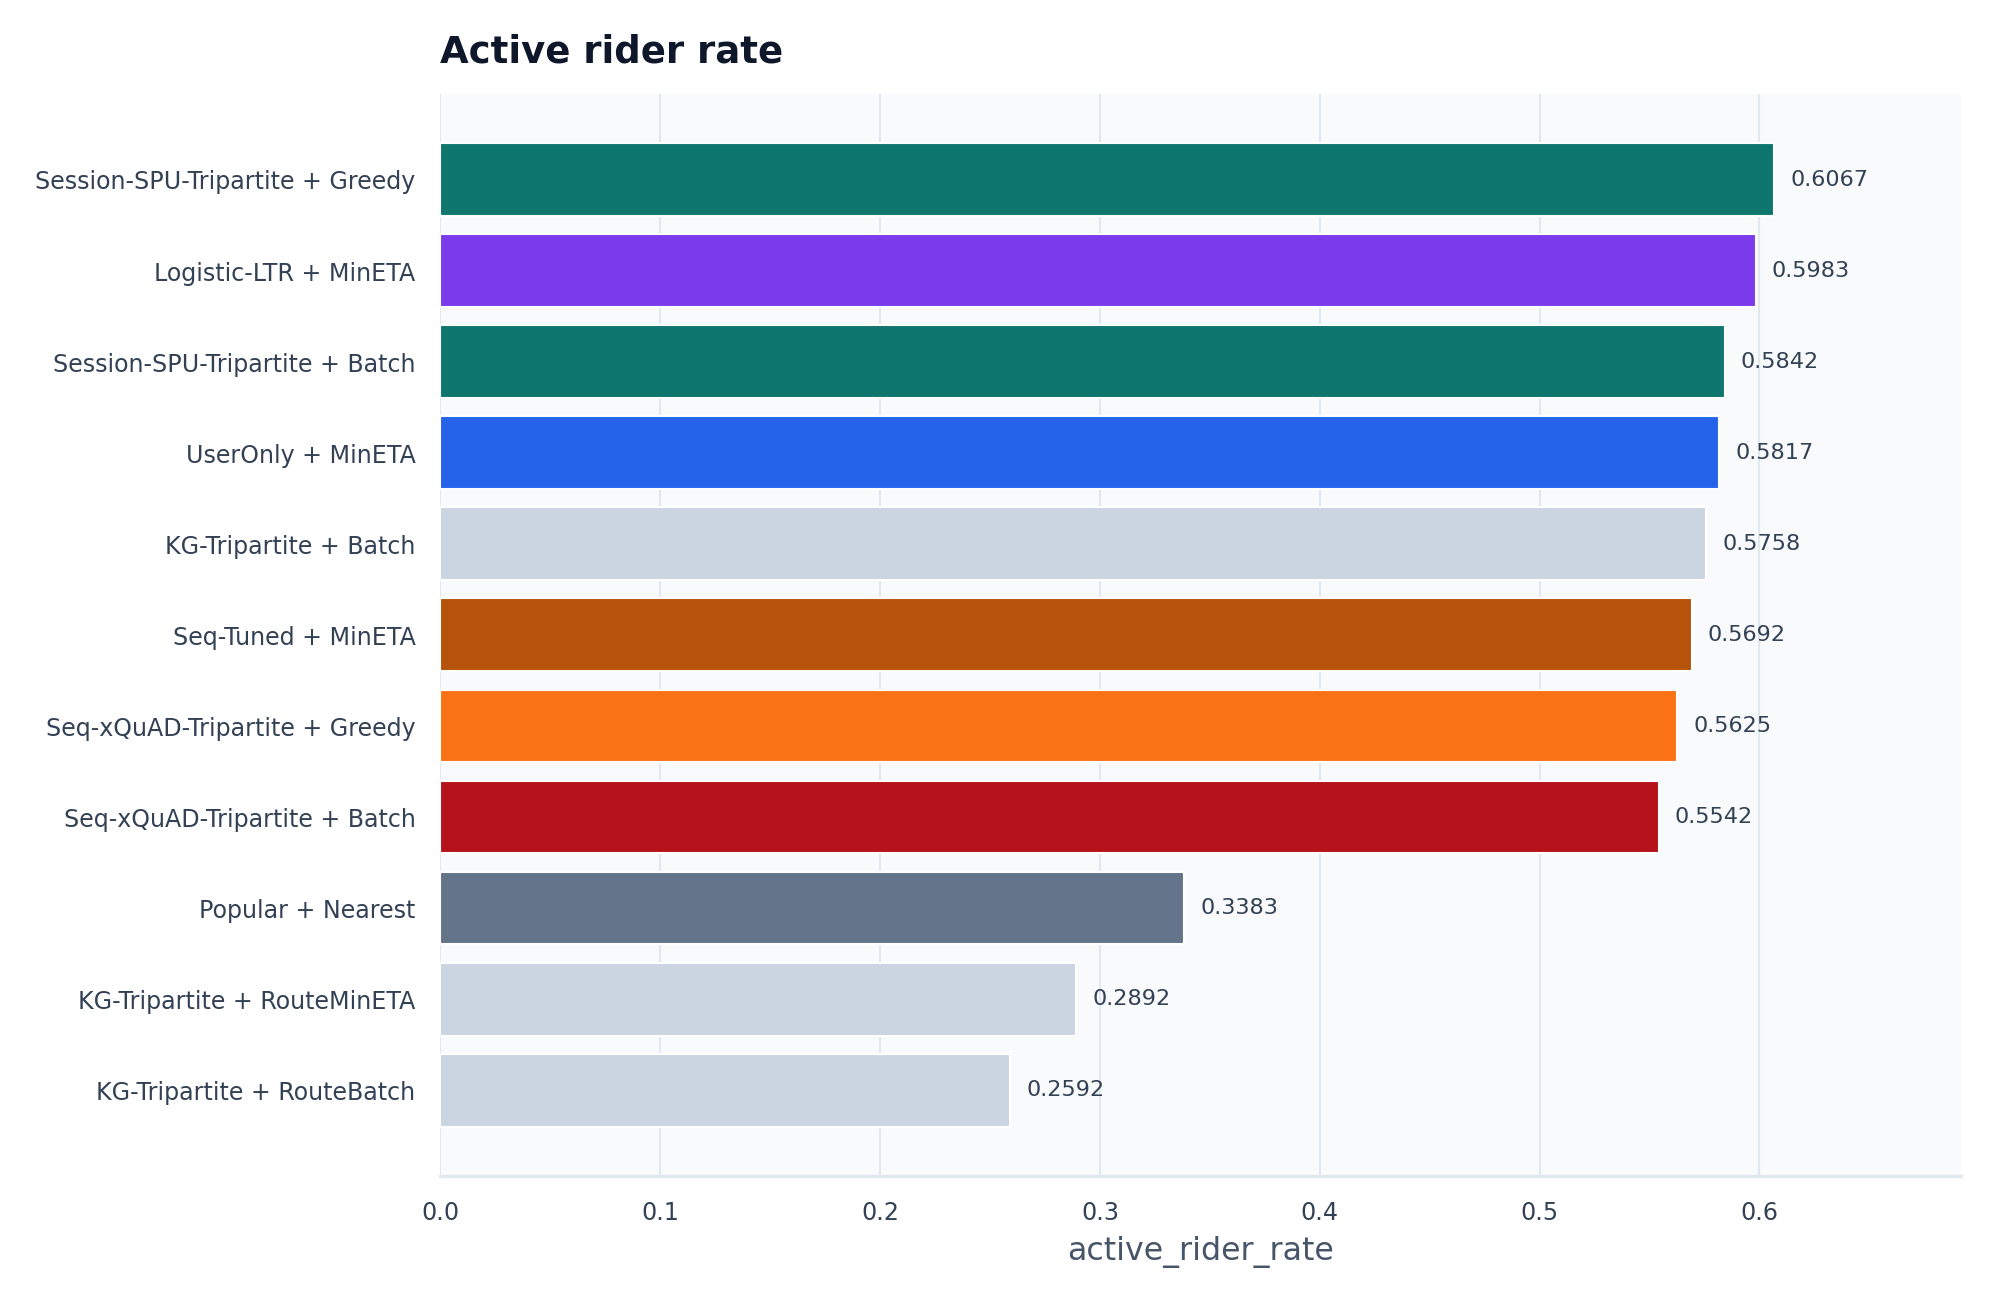
\includegraphics[width=\linewidth]{../../outputs/figures/simulation_active_rider_rate.png}
            \caption{活跃骑手率对比}
            \label{fig:active_rider}
        \end{subfigure}
        \hfill
        \begin{subfigure}{0.48\linewidth}
            \centering
            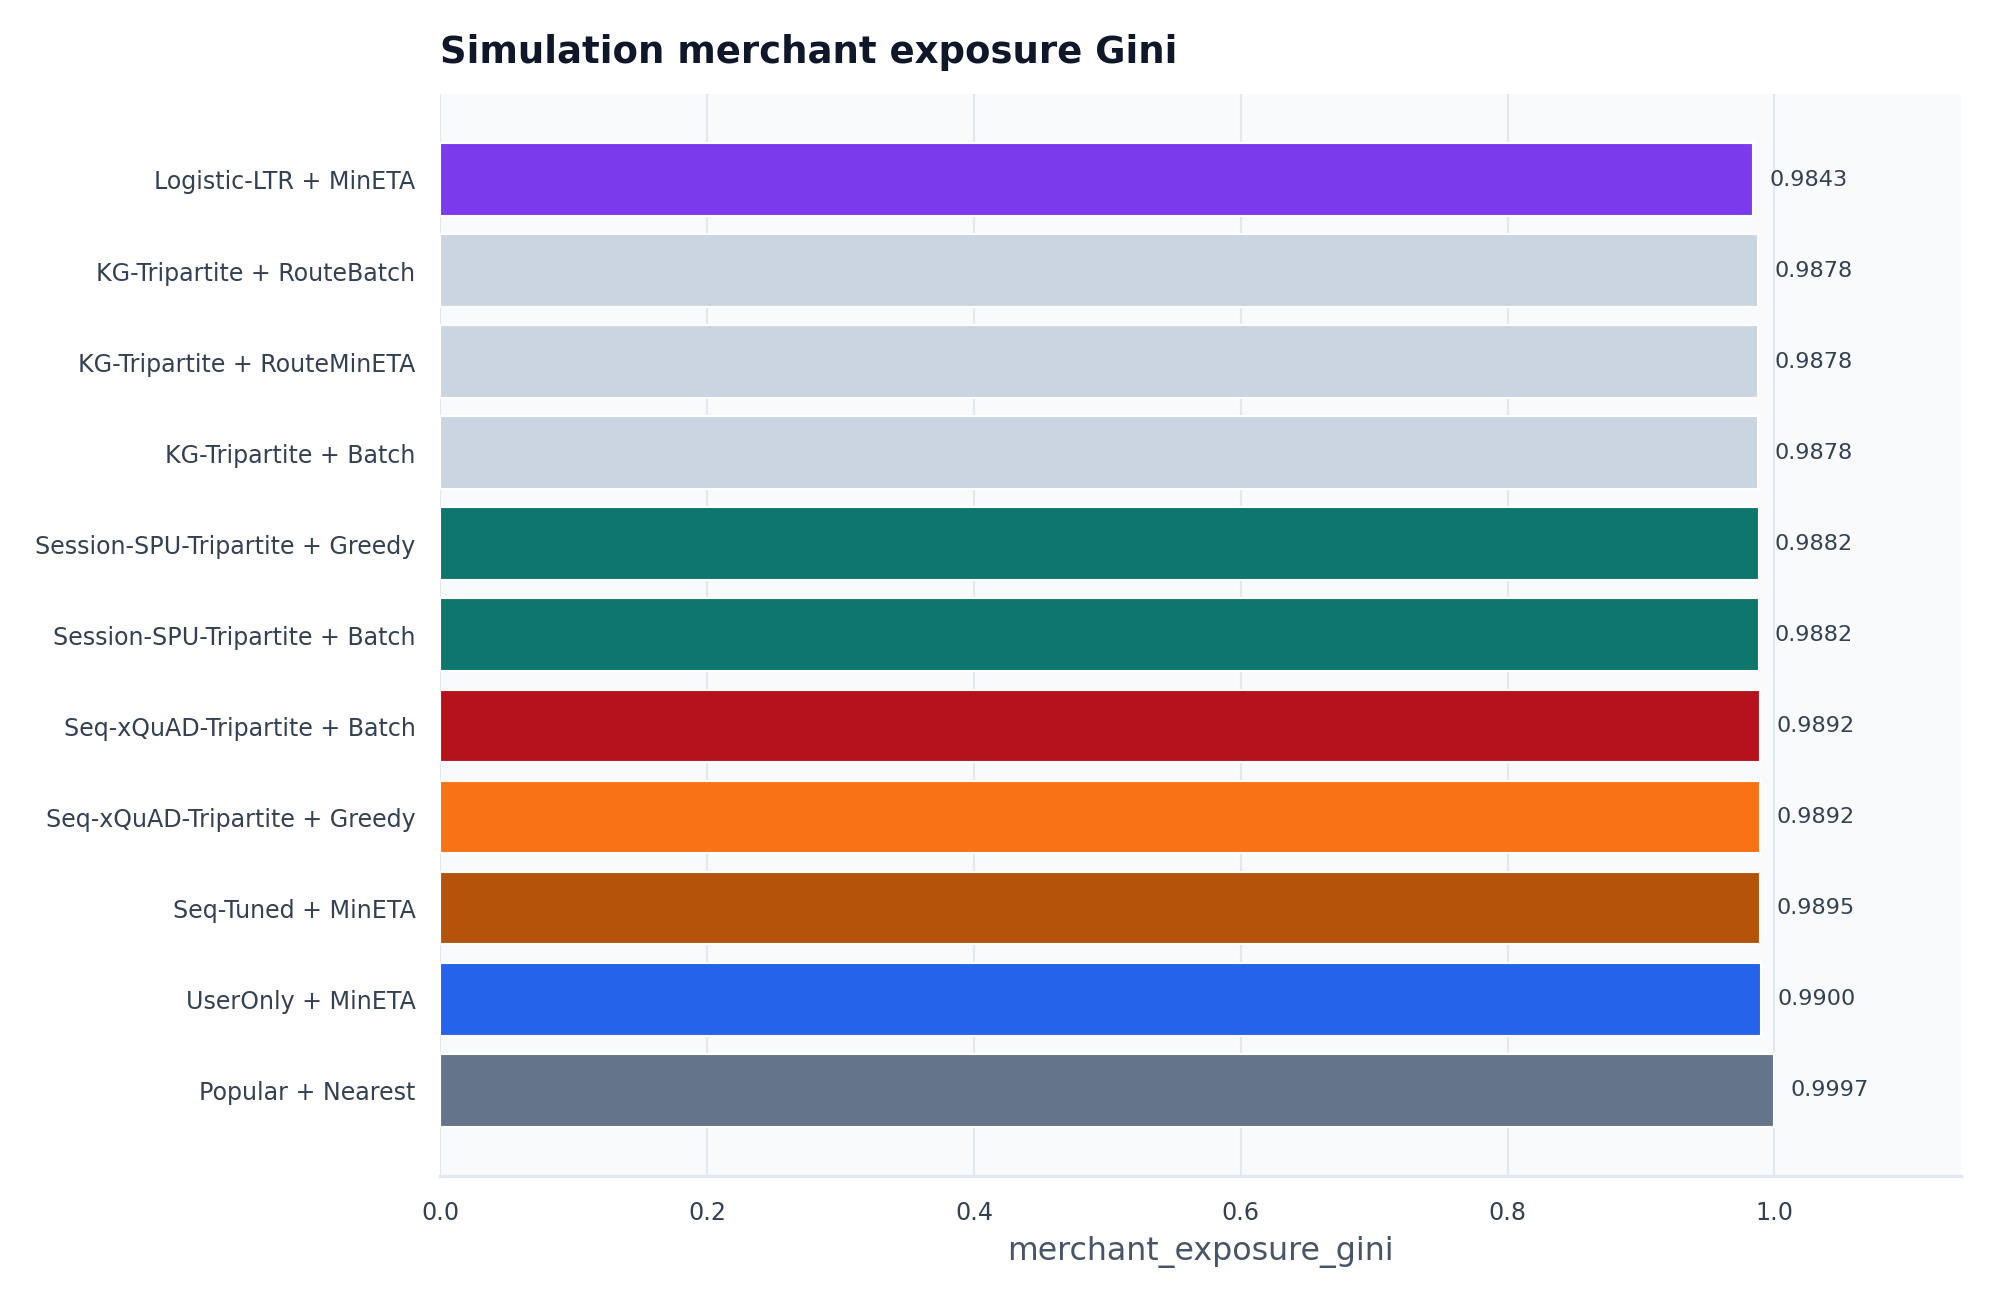
\includegraphics[width=\linewidth]{../../outputs/figures/simulation_exposure_gini.png}
            \caption{仿真中商家曝光 Gini 对比}
            \label{fig:sim_exposure_gini}
        \end{subfigure}
        \caption{骑手活跃率与商家曝光公平性}
        \label{fig:sim_rider_merchant}
    \end{figure}

    图 \ref{fig:rider_metrics} 展示了骑手侧指标。负载感知的派单策略（load\_aware）在骑手负载均衡和收入公平性上均优于 nearest 和 min\_eta。图 \ref{fig:sim_rider_merchant} 显示三方策略在保持较高活跃骑手率的同时，商家曝光 Gini 也更低。

    \subsection{三方帕累托前沿分析}

    为综合评估推荐准确率与系统效用之间的权衡，图 \ref{fig:pareto} 将各策略映射到 Recall@20（推荐侧）与平台效用（系统侧）的二维空间中，并标注帕累托前沿。

    \begin{figure}[htbp]
        \centering
        \begin{subfigure}{0.48\linewidth}
            \centering
            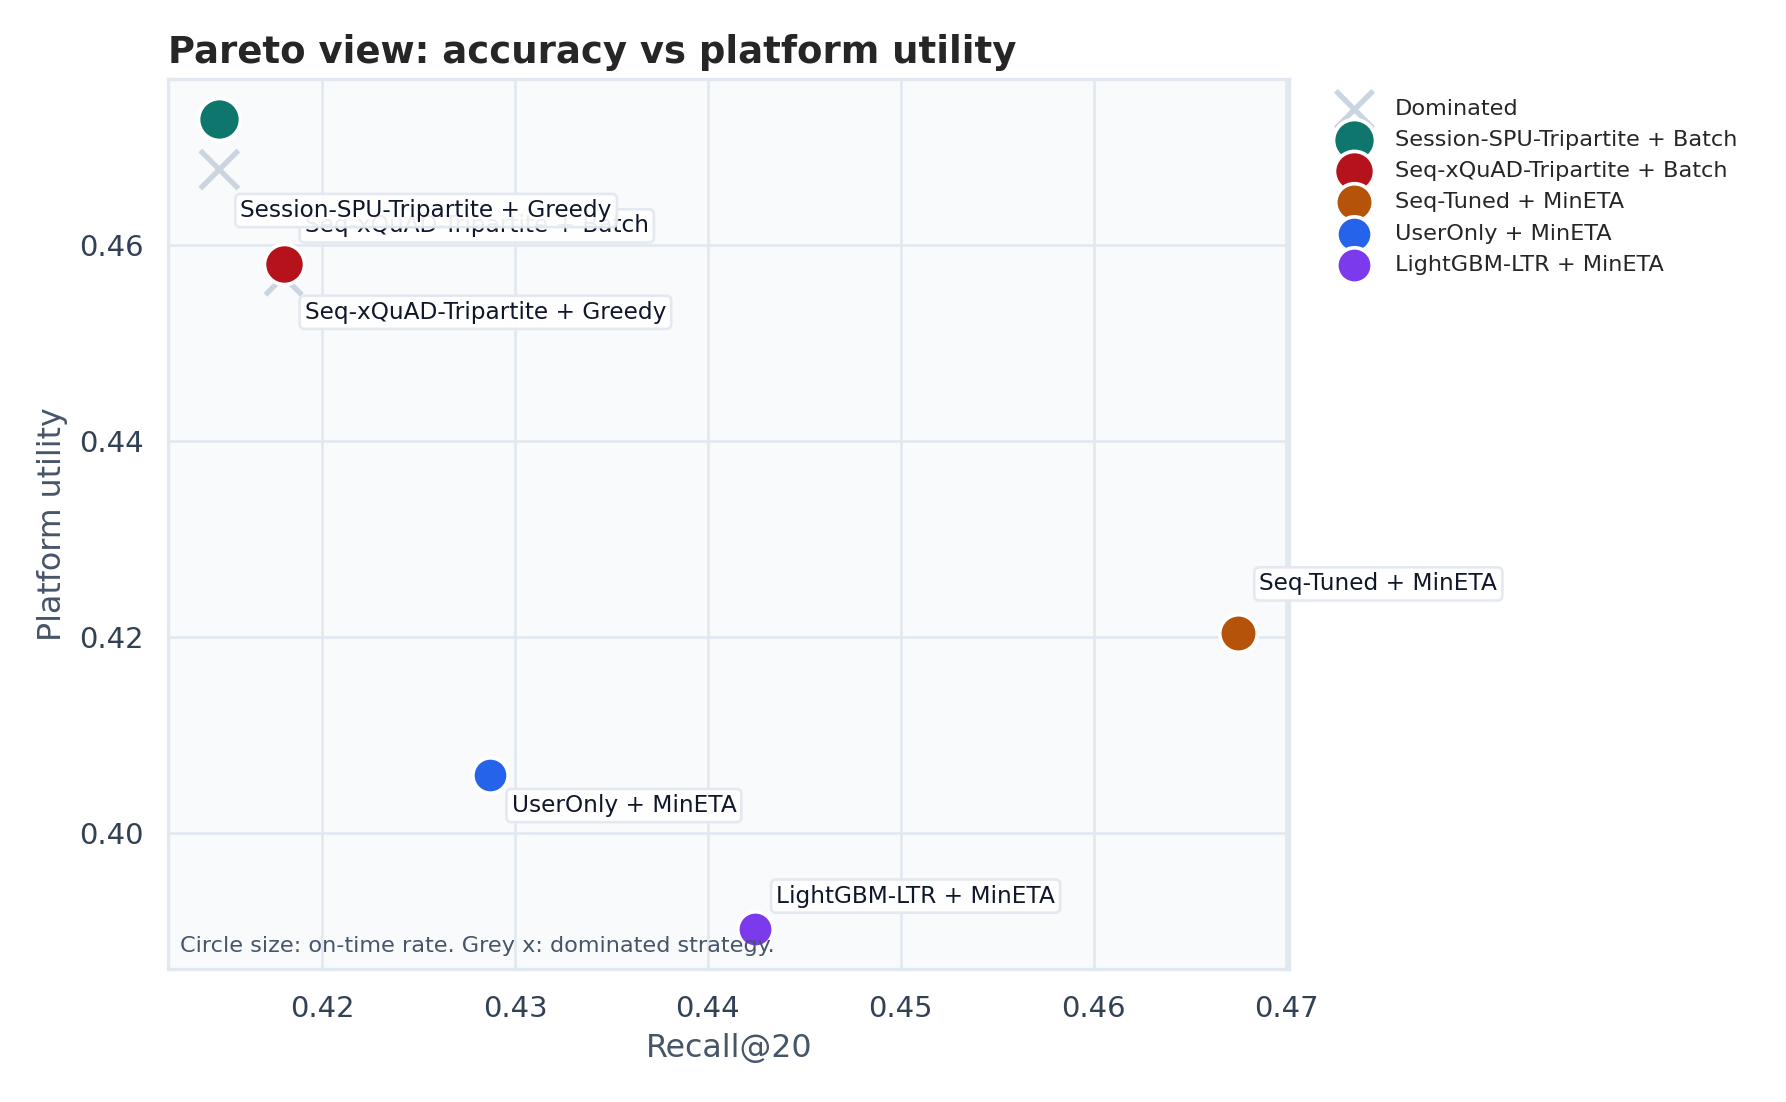
\includegraphics[width=\linewidth]{../../outputs/figures/pareto_recall_utility.png}
            \caption{Recall@20 与平台效用的帕累托前沿}
            \label{fig:pareto}
        \end{subfigure}
        \hfill
        \begin{subfigure}{0.48\linewidth}
            \centering
            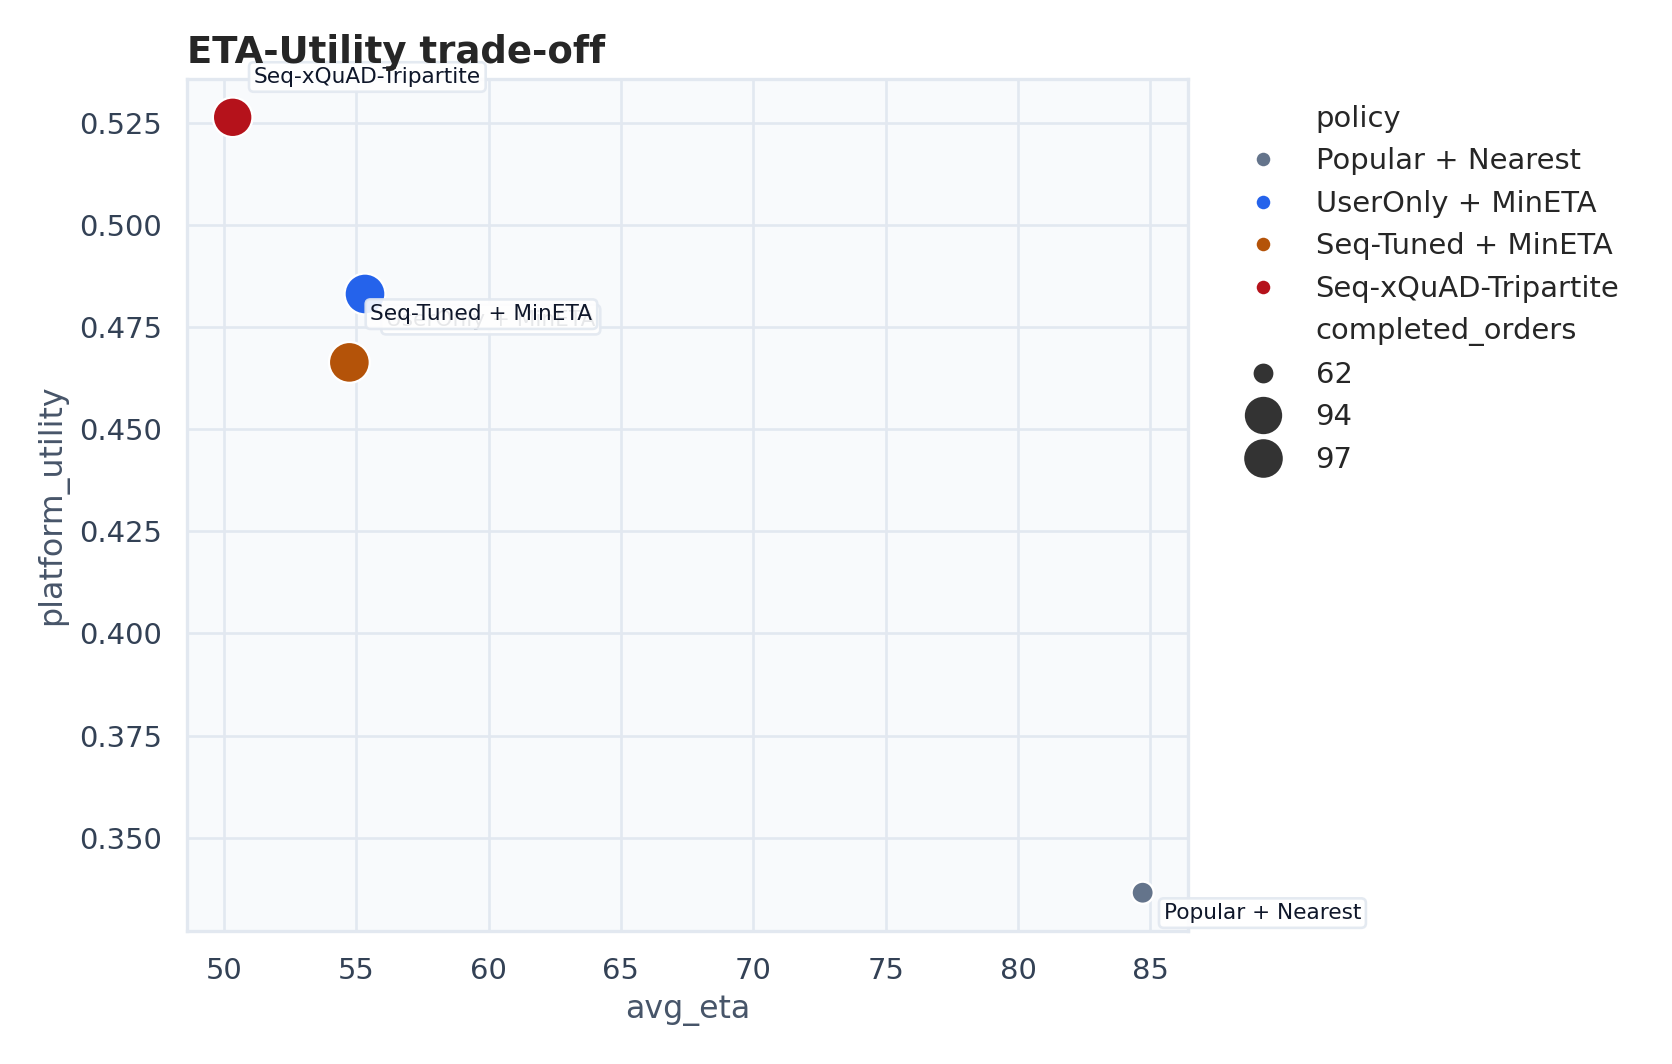
\includegraphics[width=\linewidth]{../../outputs/figures/tradeoff_eta_utility.png}
            \caption{平均 ETA 与平台效用的权衡}
            \label{fig:eta_utility}
        \end{subfigure}
        \caption{三方权衡与帕累托前沿分析}
        \label{fig:tripartite_tradeoff}
    \end{figure}

    \begin{figure}[htbp]
        \centering
        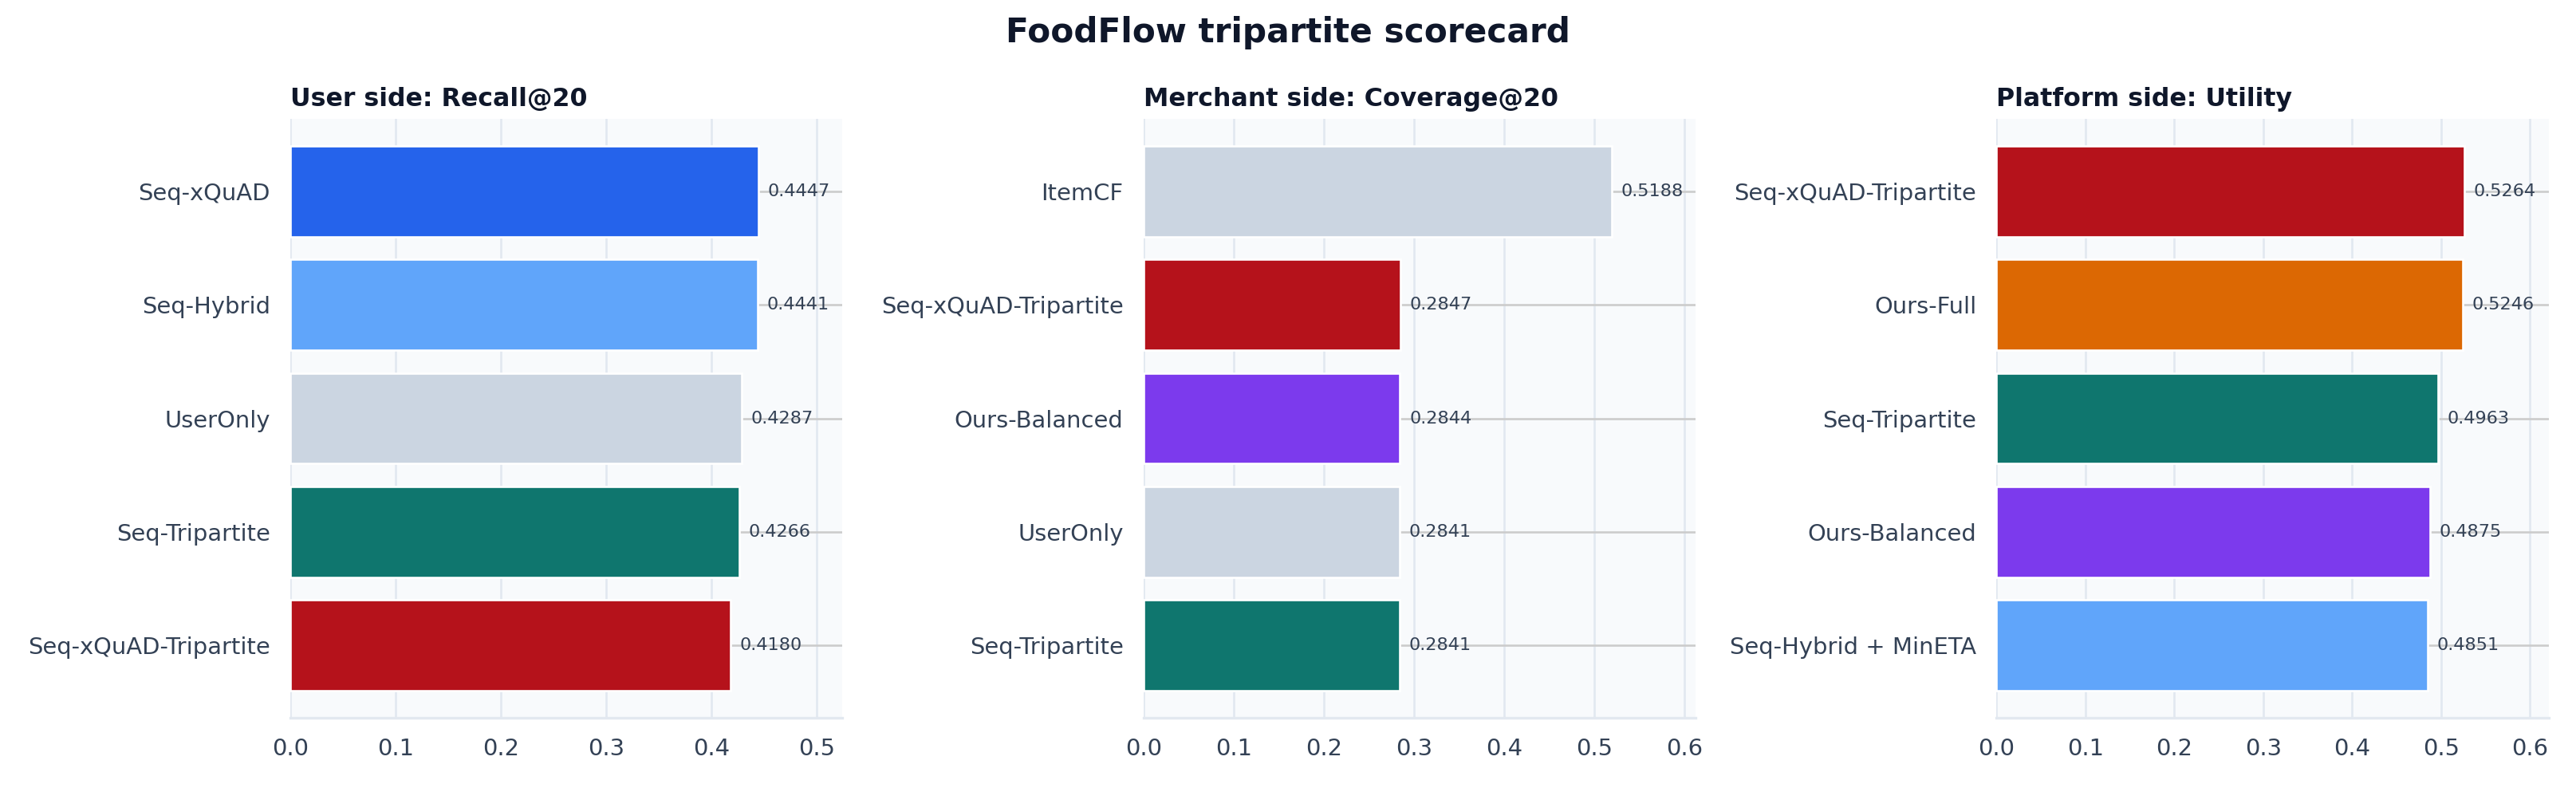
\includegraphics[width=0.7\linewidth]{../../outputs/figures/tripartite_scorecard.png}
        \caption{三方策略综合记分卡}
        \label{fig:scorecard}
    \end{figure}

    从图 \ref{fig:pareto} 可以清晰识别三类前沿策略：
    \begin{itemize}
        \item \textbf{离线准确率前沿：}Seq-Tuned 和 LightGBM-LTR 代表推荐准确率的上界，在 Recall@20 上分别达到 0.4675 和 0.4424。
        \item \textbf{系统效用前沿（常规运力）：}Session-SPU-Tripartite、Seq-xQuAD-Tripartite（Batch）和 KG-Tripartite 代表平台效用的上界，分别达到 0.557、0.553 和 0.550。
        \item \textbf{系统效用前沿（运力紧张）：}KG-Tripartite + RouteMinETA 在压力场景下平台效用达到 0.544，远超同场景下最优槽位匹配的 0.486，说明路径感知顺路派单是高峰爆单时的韧性机制。
    \end{itemize}

    这两类策略共同构成了三方推荐的权衡边界——说明在外卖推荐场景中，纯粹的准确率优化和系统级多目标优化并不完全重合，需要根据平台的战略偏好进行折中。图 \ref{fig:scorecard} 的综合记分卡进一步印证了这一发现：三方模型在配送时效和平台效用上表现优异，而 Seq-Tuned 在用户侧指标上保持领先。

    \section{实验感想}

    通过本实验，我们构建了完整的"推荐—重排—履约仿真"闭环系统，获得以下主要收获：

    \begin{enumerate}
        \item \textbf{推荐系统需要从系统视角评估。}离线准确率指标（Recall、NDCG）只能反映模型匹配用户历史行为的能力，无法衡量推荐结果对履约链路的下游影响。FoodFlow 通过引入动态履约仿真，揭示了推荐准确率与平台效用之间的权衡关系。
        \item \textbf{三方重排在履约指标上带来了显著收益。}在候选排序中纳入商家公平、ETA 和供给约束，虽然会略微牺牲离线准确率，但能显著降低平均 ETA 和超时率，提升平台全局效用。这一发现对实际外卖平台的推荐系统设计具有启示意义。
        \item \textbf{知识图谱信号能增强三方推荐的排序精度与可解释性。}KG-Tripartite 在三方模型中离线准确率最高（Recall@20=0.4342、NDCG@20=0.3492），同时通过品类/商圈/价位结构化路径提供可解释推荐证据。kg-demo 子项目的完整动态 KG 注意力模型进一步验证了时间衰减图谱信号与协同过滤的互补性。
        \item \textbf{二分图批量匹配优于贪心逐单分配。}匈牙利算法在容量约束下寻求全局最优匹配，相比贪心策略能更均衡地分配骑手负载，降低超时风险。
        \item \textbf{路径感知顺路派单是高峰爆单时的韧性机制。}运力充足时，槽位批量匹配的 ETA 更优；但在运力紧张（30 骑手）的压力场景下，cheapest-insertion 顺路派单大幅反超——平均 ETA 比最优槽位匹配低约 16 分钟，顺路接单率达 66.9\%。派单机制可随供需状态切换，这是三方联合视角的核心论据。
        \item \textbf{多种子仿真为策略比较提供了统计置信度。}10 种子均值和 95\% 置信区间的使用使得策略间差异的显著性可以被量化评估，避免了单种子点估计的偶然性。
        \item \textbf{真实城市地理编码使仿真具备物理意义。}通过 LaDe 数据集将用户/商家嵌入真实城市配送 GPS 分布，距离与 ETA 具备了真实街区尺度，使仿真结果不再停留于抽象数值。
    \end{enumerate}

    本实验也存在以下局限性：
    \begin{itemize}
        \item 骑手数据默认来自合成仿真，虽然可使用 LaDe delivery CSV 校准末端配送参数，但仍不能替代工业级外卖派单数据。
        \item 离线评估默认只使用前 300 名测试用户（全量测试用户约 108,739 名），大规模评估的计算开销较大。
        \item LightGBM-LTR 当前使用项目构造的候选集和特征，训练标签来自历史下单集合，后续可引入更丰富的上下文特征、真实曝光/点击标签和跨城市验证。
        \item 仿真中的 MNL 选择模型为简化的用户行为假设，实际用户的下单决策受更多因素影响。
        \item KG-Tripartite 主模型使用的是免训练的轻量图谱近似（时间衰减 + 关系加权匹配）；完整的动态 KG 注意力模型与 GPU 实验结果在 kg-demo/ 子项目中，两者共用 TRD 数据但尚未在统一仿真框架下直接对比。
        \item 当前三方优化采用"推荐重排 + 下单后骑手匹配"的解耦闭环，不是工业级端到端联合调度系统。
    \end{itemize}

    总体而言，FoodFlow 验证了"推荐 + 履约联合优化"这一技术路线的可行性。后续工作可以围绕更精细的骑手行为建模（如接单意愿学习、多平台竞争）、完整 KG 注意力模型与三方重排的端到端融合、更大规模的真实数据验证以及在线 A/B 测试展开。


\end{document}
